\documentclass[10pt,letterpaper]{article} % {{{
\usepackage[top=0.85in,left=2.75in,footskip=0.75in]{geometry}
\usepackage{amsmath,amssymb}
% Use adjustwidth environment to exceed column width (see example table in text)
\usepackage{changepage}

% textcomp package and marvosym package for additional characters
\usepackage{textcomp,marvosym}
\usepackage{subcaption}


% cite package, to clean up citations in the main text. Do not remove.
\usepackage{cite}

% Use nameref to cite supporting information files (see Supporting Information section for more info)
\usepackage{nameref,hyperref}

% line numbers
\usepackage[right]{lineno}

% ligatures disabled
\usepackage[nopatch=eqnum]{microtype}
\DisableLigatures[f]{encoding = *, family = * }

% color can be used to apply background shading to table cells only
\usepackage[table]{xcolor}

% array package and thick rules for tables
\usepackage{array}

% create "+" rule type for thick vertical lines
\newcolumntype{+}{!{\vrule width 2pt}}

% create \thickcline for thick horizontal lines of variable length
\newlength\savedwidth
\newcommand\thickcline[1]{%
  \noalign{\global\savedwidth\arrayrulewidth\global\arrayrulewidth 2pt}%
  \cline{#1}%
  \noalign{\vskip\arrayrulewidth}%
  \noalign{\global\arrayrulewidth\savedwidth}%
}

% \thickhline command for thick horizontal lines that span the table
\newcommand\thickhline{\noalign{\global\savedwidth\arrayrulewidth\global\arrayrulewidth 2pt}%
\hline
\noalign{\global\arrayrulewidth\savedwidth}}


% Remove comment for double spacing
%\usepackage{setspace} 
%\doublespacing

% Text layout
\raggedright
\setlength{\parindent}{0.5cm}
\textwidth 5.25in 
\textheight 8.75in

% Bold the 'Figure #' in the caption and separate it from the title/caption with a period
% Captions will be left justified
\usepackage[aboveskip=1pt,labelfont=bf,labelsep=period,justification=raggedright,singlelinecheck=off]{caption}
\renewcommand{\figurename}{Fig}
\renewcommand{\succ}{\textrm{succ}}

\newcommand{\fref}[1]{Fig.~\ref{#1}}
\newcommand{\eref}[1]{eq.~(\ref{#1})}
% Use the PLoS provided BiBTeX style
\bibliographystyle{plos2015}

% Remove brackets from numbering in List of References
\makeatletter
\renewcommand{\@biblabel}[1]{\quad#1.}
\makeatother



% Header and Footer with logo
\usepackage{lastpage,fancyhdr,graphicx}
\usepackage{epstopdf}



\usepackage[english]{babel}
\usepackage{graphicx,helvet}
\usepackage{color}
\usepackage{url}
\usepackage{amssymb}
\usepackage[utf8]{inputenc}
\usepackage{hyperref}
\usepackage[inline]{showlabels}
\usepackage{bbm,bm}
\usepackage{soul}
\usepackage{amsfonts}
\usepackage{showlabels}

\usepackage{tikz}
\usetikzlibrary{arrows}
\usetikzlibrary{quantikz}

\usepackage[draft,inline,nomargin]{fixme} \fxsetup{theme=color}
\FXRegisterAuthor{cp}{acp}{\color{blue}CP}
\FXRegisterAuthor{tb}{ttb}{\color{green}TB}




%\pagestyle{myheadings}
\pagestyle{fancy}
\fancyhf{}
%\setlength{\headheight}{27.023pt}
%\lhead{\includegraphics[width=2.0in]{PLOS-submission.eps}}
\rfoot{\thepage/\pageref{LastPage}}
\renewcommand{\headrulewidth}{0pt}
\renewcommand{\footrule}{\hrule height 2pt \vspace{2mm}}
\fancyheadoffset[L]{2.25in}
\fancyfootoffset[L]{2.25in}
\lfoot{\today}

%% Include all macros below

\newcommand{\lorem}{{\bf LOREM}}
\newcommand{\ipsum}{{\bf IPSUM}}
\DeclareMathOperator{\tr}{tr}
\newtheorem{definition}{Definition}
\newtheorem{theorem}{Theorem}

%% END MACROS SECTION

% }}}
\begin{document}
% Titulo, afiliacion, abstract  {{{
\vspace*{0.2in}

% Title must be 250 characters or less.


\begin{flushleft}
{\Large
\textbf\newline{Title of submission to PLOS journals} % Please use "sentence case" for title and headings (capitalize only the first word in a title (or heading), the first word in a subtitle (or subheading), and any proper nouns).
}
\newline
% Insert author names, affiliations and corresponding author email (do not include titles, positions, or degrees).
\\
Tomás Basile\textsuperscript{1\Yinyang},
Carlos Pineda\textsuperscript{2*\Yinyang},
\\
\bigskip
\textbf{1} Facultad de Ciencias. Universidad Nacional Autónoma de México, Ciudad de México 01000, Mexico
\\
\textbf{2} Instituto de Física, Universidad Nacional Autónoma de México, Ciudad de México 01000, México
\\
\bigskip

% Insert additional author notes using the symbols described below. Insert symbol callouts after author names as necessary.
% 
% Remove or comment out the author notes below if they aren't used.
%
% Primary Equal Contribution Note
\Yinyang These authors contributed equally to this work.

% Additional Equal Contribution Note
% Also use this double-dagger symbol for special authorship notes, such as senior authorship.
% \ddag These authors also contributed equally to this work.

% Current address notes
% \textcurrency Current Address: Dept/Program/Center, Institution Name, City, State, Country % change symbol to "\textcurrency a" if more than one current address note
% \textcurrency b Insert second current address 
% \textcurrency c Insert third current address

% Deceased author note
% \dag Deceased

% Group/Consortium Author Note
% \textpilcrow Membership list can be found in the Acknowledgments section.

% Use the asterisk to denote corresponding authorship and provide email address in note below.
* carlospgmat03@gmail.com

\end{flushleft}
% Please keep the abstract below 300 words
\section*{Abstract}
Lorem ipsum dolor sit amet, consectetur adipiscing elit. Curabitur eget porta erat. Morbi consectetur est vel gravida pretium. Suspendisse ut dui eu ante cursus gravida non sed sem. Nullam sapien tellus, commodo id velit id, eleifend volutpat quam. Phasellus mauris velit, dapibus finibus elementum vel, pulvinar non tellus. Nunc pellentesque pretium diam, quis maximus dolor faucibus id. Nunc convallis sodales ante, ut ullamcorper est egestas vitae. Nam sit amet enim ultrices, ultrices elit pulvinar, volutpat risus.


% Please keep the Author Summary between 150 and 200 words
% Use first person. PLOS ONE authors please skip this step. 
% Author Summary not valid for PLOS ONE submissions.   
%\section*{Author summary}
%Lorem ipsum dolor sit amet, consectetur adipiscing elit. Curabitur eget porta erat. Morbi consectetur est vel gravida pretium. Suspendisse ut dui eu ante cursus gravida non sed sem. Nullam sapien tellus, commodo id velit id, eleifend volutpat quam. Phasellus mauris velit, dapibus finibus elementum vel, pulvinar non tellus. Nunc pellentesque pretium diam, quis maximus dolor faucibus id. Nunc convallis sodales ante, ut ullamcorper est egestas vitae. Nam sit amet enim ultrices, ultrices elit pulvinar, volutpat risus.

\linenumbers

% Use "Eq" instead of "Equation" for equation citations.
% }}}
\section{Introduction} % {{{
\tbnote{Poner intro luego. Ver libro de writing science}


% }}}
\section{Pauli channels and dynamical maps}  \label{sec: Pauli Channels} % {{{
% Intro  {{{
% \textbf{Lista de puntos:}
% \begin{itemize}
% \item \textbf{Circuit for a Pauli channel:}  Propose a circuit to simulate a Pauli channel on $n$ qubits. It works by creating a $2n$-qubit state on ancilla qubits.
% \item \textbf{Simulation:} Show the fidelities of simulating the circuit on a quantum computer for many one-qubit channels inside the tetrahedron.
% \item \textbf{For Pauli dynamical maps}: See how the circuit generalizes to parametrized channels and notice that many rotations are needed to create the $2n$-ancilla qubit state. \\
% \end{itemize}

In this section  we introduce the concept of quantum channels, focusing on a
specific type called Pauli channels.  Furthermore, we define Pauli dynamical
maps, which are curves of Pauli channels parametrized by a variable.
% }}}
\subsection{Quantum Channels} \label{subsec: Quantum Channels} % {{{


In quantum mechanics, a closed system's state is represented by a vector in a
Hilbert space $\mathcal{H}$.  The state's evolution is unitary and given by
Schrodinger's equation~\cite{Rieffel}.  However, in real-world situations,
quantum systems are usually open, which means that they interact with their
environment~\cite{Breuer}.  For instance, the system's state may become
entangled with the environment, leading to a loss of information about the
system's state over time.

To describe open systems, instead of state vectors, we use matrices $\rho$ that
act on $\mathcal{H}$.  These matrices are called density matrices, and they
include information about the system's interaction with its environment.  For a
density matrix $\rho$ to be physically valid, it must satisfy two conditions:
$\tr(\rho) = 1$ and it must be positive semi-definite, which is denoted as
$\rho \geq 0$~\cite{chuangbook}.


Knowing this, we can now define quantum channels.  Quantum channels are
operators $\mathcal{E}$ that can describe the evolution of open quantum
systems, such that $\rho \rightarrow \mathcal{E}(\rho)$.  Quantum channels are
the most general linear operations that a quantum system can undergo
independently of its past~\cite{zimansbook,cirac}.  These channels are
constructed based on three fundamental properties: linearity, trace
preservation, and complete positivity.

Linearity ensures that a quantum channel $\mathcal{E}$ maps any ensemble of
density matrices into the corresponding ensemble of their evolution.  The trace
preserving property is given by $\tr (\mathcal{E}[\rho]) = \tr (\rho) = 1$ and
guarantees that the quantum channel does not change the condition that
$\tr(\rho) = 1$.  Finally, the channel should also preserve the condition $\rho
\geq 0$, and a map that does this is called a positive map.  However,
positivity of $\mathcal{E}$ is not enough, and we actually require the more
restrictive condition of complete positivity.  Complete positivity means that
$\mathcal{E} \otimes \mathbb{I}_n$ is positive for any positive integer $n$
(where $\mathbb{I}_n$ is the $n\times n$ identity matrix).  This ensures that
even if the principal system is entangled with another system, applying
$\mathcal{E}$ to the principal system while doing nothing to the other one
still results in  a positive semidefinite state for the principal
system~\cite{chuangbook}. 

Given a quantum channel $\mathcal{E}$, the condition of trace preservation is
straightforward to verify but complete positivity is not as simple.  To test
complete positivity of a quantum channel, Jamiołkowski and
Choi~\cite{choi,jamil} developed a simple algorithm that exploits the
isomorphism between a channel $\mathcal{E}$ and the state $\mathcal{D} =
(\mathbb{I} \otimes \mathcal{E}) [|\Omega \rangle \langle  \Omega|]$, where
$|\Omega\rangle = 1/\text{dim}(\mathcal{H}) \sum_{i}^{\text{dim}(\mathcal{H})}
|i \rangle |i \rangle$ is a maximally entangled state between the original
system and an ancilla.  Remarkably, the map $\mathcal{E}$ is completely
positive if and only if $\mathcal{D}$ (also known as the Choi or dynamical
matrix of $\mathcal{E}$) is positive semidefinite.

% }}}
\subsection{Pauli Channels}  \label{subsec: Pauli Channels} % {{{

We have discussed the main features of quantum channels and 
now we turn our attention to a specific 
type of channels for $N$-qubit systems called Pauli channels.
First we will define these channels for single-qubit systems,
whose most general density matrix can be written as~\cite{chuangbook}:
\begin{equation}
\label{eq: Density Matrix}
\rho = \dfrac{1}{2} \sum_{\alpha=0}^{3} r_{\alpha} \sigma_{\alpha},
\end{equation}
with $\sigma_0 = \mathbb{I}$, and $\sigma_{1,2,3}$ the usual Pauli matrices.
The condition $\tr(\rho) = 1$ requires that $r_0 = 1$ while $\rho \geq 0$ 
implies that the remaining $r_{1,2,3}$ form
a vector $\vec{r}= (r_1,r_2,r_3)$ inside a unit sphere known as the Bloch sphere~\cite{Marinescu}.
That is, every possible density matrix for a one-qubit
system is uniquely associated with a point in a unit sphere. 
% \cpnote{explicar un poco mejor. Me parece que para el publico vale 
% la pena ser un poco mas explicito. pero no estoy muy seguro.}

Given a one-qubit system described by $\rho$, 
a Pauli channel is defined as an operation that with probability $k_{\gamma}$
applies the Pauli matrix $\sigma_{\gamma}$ to
the system, for $\gamma = 0,1,2,3$~\cite{geometry}.
Mathematically, the Pauli channel is written in the following way:
\begin{eqnarray}
\label{eq: Pauli channel 1 qbit}
\mathcal{E}(\rho) = \sum_{\gamma=0}^3 k_{\gamma} \sigma_{\gamma} \rho \sigma_{\gamma},
\end{eqnarray} 
where the probabilities $k_{\gamma}$ of applying $\sigma_{\gamma}$
are non-negative real numbers such that 
$\sum_{\gamma} k_{\gamma} = 1$ (these conditions also ensure that the channel is 
trace preserving and completely positive).

Pauli channels are some of the 
most fundamental noise models in quantum information science~\cite{Terhal}. 
Some notable examples of Pauli channels are the following:
\begin{itemize}
\item \textbf{Bit Flip Channel:} This is a channel that with probability $1-p$ leaves the qubit as it is 
and with probability $p$ it applies the $\sigma_1$ matrix 
(which flips the basis states $|0\rangle$ and $|1\rangle$ of the qubit), and
so it is given by:
\begin{align*}
\mathcal{E}(\rho) = (1-p) \rho + p \sigma_1 \rho \sigma_1.
\end{align*}
Analogous channels exist using $\sigma_3$ (called the bit flip channel,
which has a probability $p$ of adding a relative phase $\pi$ to the state) or 
using $\sigma_2$ (called the phase flip channel, 
which has a probability $p$ of 
flipping the base states and also add a relative phase $\pi$).
\item \textbf{Depolarizing channel:} 
This channel has a probability $1-p$
of doing nothing to the qubit and a probability $p$ of converting it into the maximally mixed state $\dfrac{1}{2} \mathbb{I}$
and it can be written as:
\begin{equation}
\mathcal{E}(\rho) = (1-p)\rho + p \dfrac{1}{2} \mathbb{I} = \left(1 - \dfrac{3p}{4} \right) \sigma + \dfrac{p}{4} \sigma_1 \rho \sigma_1 + \dfrac{p}{4} \sigma_2 \rho \sigma_2+ \dfrac{p}{4} \sigma_3 \rho \sigma_3.
\end{equation} 
\end{itemize}

We can also see how an arbitrary Pauli channel acts on an arbitrary  
density matrix.
To do it, we substitute \eref{eq: Density Matrix} 
in \eref{eq: Pauli channel 1 qbit}:
\begin{equation}
\mathcal{E}(\rho) = \dfrac{1}{2}\sum_{\gamma,\alpha=0}^3 k_{\gamma} r_{\alpha} \sigma_{\gamma} \sigma_{\alpha} \sigma_{\gamma}.
\end{equation}
This can be simplified by using the following property of Pauli matrices:
\begin{equation}
\label{eq: propiedad-pauli}
\sigma_{\gamma} \sigma_{\alpha} \sigma_{\gamma} = A_{\alpha,\gamma} \sigma_{\alpha}, \;\;\;\;\; \text{with} \; A_{\alpha,\gamma} = \begin{pmatrix}
1 & 1 & 1 & 1\\
1 & 1 & -1 &-1 \\
1 & -1 & 1 & -1 \\
1 & -1 & -1 & 1
\end{pmatrix},
\end{equation}
which leads to
\begin{equation}
\label{eq: rho-transformada}
\mathcal{E}(\rho) = \dfrac{1}{2} \sum_{\alpha} \left(\sum_{\gamma} A_{\alpha, \gamma} k_{\gamma} \right) r_{\alpha} \sigma_{\alpha}.
\end{equation}
\eref{eq: rho-transformada} once again has the form of \eref{eq: Density Matrix}
but with components $\left( \sum_{\gamma} A_{\alpha,\gamma} k_{\gamma} \right) r_{\alpha}$.
This gives us another way of understanding Pauli channels
as operations that take each component $r_{\alpha}$
of the density matrix and multiplies them
by $\sum_{\gamma} A_{\alpha,\gamma} k_{\gamma}$, 
that is:
\begin{equation}
\label{eq: multipliers}
r_{\alpha}  \xrightarrow[\text{Channel}]{\text{Pauli}}  \tau_{\alpha} r_{\alpha} ,\;\; \tau_{\alpha} := \sum_{\gamma} A_{\alpha,\gamma} k_{\gamma}.
\end{equation}
Notice that $\tau_0 = 1$, which is a consequence of $\sum_{\gamma}k_{\gamma}=1$
and ensures that after the channel, the resulting density matrix still has trace one. 
Furthermore, reverting the definition of $\tau_{\alpha}$ by using that $A^{-1} = \dfrac{1}{4} A$, 
we get that $k_{\gamma} = \dfrac{1}{4} \sum_{\alpha} A_{\alpha,\gamma} \tau_{\alpha}$.
Then, using that $k_{\gamma} \geq 0$
we get the following conditions on the multipliers $\tau_{\alpha}$:
\begin{eqnarray}
\label{eq: conditions-tetrahedron}
&1+\tau_i -\tau_j - \tau_k \geq 0,  \;\;\; \text{for $i,j,k$ different numbers in $\{1,2,3\}$}, \\
&1+\tau_1 + \tau_2 + \tau_3 \geq 0.
\end{eqnarray}

These conditions imply that $(\tau_1,\tau_2,\tau_3)$
has to be inside a tetrahedron with
vertices $(1,1,1), (1,-1,-1),(-1,1,-1)$ and $(-1,-1,1)$. 
Therefore, the $\tau_{1,2,3}$ are numbers between 
$-1$ and $1$, which means that the components
$r_{\alpha}$ of the density matrix are always 
attenuated and possibly sign flipped.

Having defined the one qubit case,  we can now generalize to $N$ qubits.
In order to do it, we need to introduce the so-called \textit{Pauli strings}, defined as
\begin{eqnarray}
\label{eq: Pauli string}
\sigma_{\vec{\alpha}} = \sigma_{\alpha_1} \otimes \sigma_{\alpha_2}\otimes \cdots \otimes \sigma_{\alpha_N},
\end{eqnarray}
where $\vec{\alpha}$ denotes a multi-index $(\alpha_1, \cdots, \alpha_N)$
 and $\alpha_i \in \{0,1,2,3\}$. 
These operators form an orthogonal basis in the space of operators acting on $N$ qubits. 
 Similarly to the single-qubit case, the density matrix $\rho$ 
of a system of $N$ qubits can be written using Pauli strings as:
\begin{equation}
\label{eq:  Density matrix Nqbit}
\rho = \dfrac{1}{2^N} \sum_{\vec{\alpha}} r_{\vec{\alpha}} \sigma_{\vec{\alpha}}.
\end{equation}
Then, just as before, we define a Pauli channel as a transformation that applies 
the operator $\sigma_{\vec{\gamma}}$ to $\rho$ with probability $k_{\vec{\gamma}}$
and is therefore described mathematically by:
\begin{equation}
\label{eq: pauli channel N-qubit}
\mathcal{E}(\rho) = \sum_{\vec{\gamma}} k_{\vec{\gamma}} \sigma_{\vec{\gamma}} \rho \sigma_{\vec{\gamma}},
\end{equation}
where just as before, $k_{\vec{\gamma}}$ are non-negative real numbers such 
that $\sum_{\vec{\gamma}} k_{\vec{\gamma}}=1$.

As in the one qubit case, Pauli channels for $N$ qubits 
attenuate the components $r_{\vec{\alpha}}$ of the density matrix.
This can be seen by substituting \eref{eq:  Density matrix Nqbit} in \eref{eq: pauli channel N-qubit}
and using the property of \eref{eq: propiedad-pauli}:
\begin{align*}
\mathcal{E}(\rho) &= \dfrac{1}{2^N} \sum_{\vec{\gamma},\vec{\alpha}} k_{\vec{\gamma}} r_{\vec{\alpha}} \sigma_{\vec{\gamma}} \sigma_{\vec{\alpha}} \sigma_{\vec{\gamma}} \\
& = \dfrac{1}{2^N} \sum_{\vec{\alpha}} \left( \sum_{\vec{\gamma}} (A^{\otimes^N})_{\vec{\alpha},\vec{\gamma}} \; k_{\vec{\gamma}} \right) r_{\vec{\alpha}} \sigma_{\vec{\alpha}},
\end{align*}
which means that applying the Pauli channel multiplies the 
components $r_{\vec{\alpha}}$ by $\tau_{\vec{\alpha}} := \sum_{\vec{\gamma}} (A^{\otimes^N})_{\vec{\alpha},\vec{\gamma}} k_{\vec{\gamma}}$.
% }}}
\subsection{Pauli Dynamical Maps} % {{{
\label{subsec: Pauli Dynamical Maps}


As seen in the last section, Pauli channels and in 
general quantum channels are discrete maps
that transform a density matrix $\rho$ into $\mathcal{E}(\rho)$.
However, we could also define a continuous set of 
channels $\varepsilon_p$ with $p$ a real parameter.

For the special case of Pauli channels, we define 
a Pauli dynamical map as a continuous parametrized 
curve drawn inside the set of Pauli channels and starting at the identity channel. 
Therefore, a Pauli dynamical map can be written as
\begin{eqnarray}
\label{eq: Pauli dynamical map}
\mathcal{E}_p(\rho) = \sum_{\vec{\gamma}} k_{\vec{\gamma}}(p) \sigma_{\vec{\gamma}} \rho \sigma_{\vec{\gamma}},
\end{eqnarray}
where $p$ is a parameter in an interval $[a,b]$ 
and $\mathcal{E}_p$ is a Pauli channel for every $p$, 
with $\mathcal{E}_a$ being the identity channel.

% }}}
% }}}
\section{Circuit for a Pauli Channel} % {{{
\label{sec: Circuit for a Pauli Channel}
% Intro {{{

In this section we propose a quantum circuit that simulates $N$-qubit Pauli
channels.  Moreover, we implement the circuit for $N=1$ on a quantum computer
and analyze the results using the diamond norm.
We find that close to the depolarizing channel, the general circuit simulator 
can implement such channels with the highest fidelity. 
% produce the highest 
% \cpnote{Quizá en una frase poner el resultado aca o ampliar
% tantito} \tbnote{Va, agregué lo siguiente: 
% We conclude that the circuit performs optimally for channels  in proximity to the
% completely depolarizing channel but
% it is deficient close to unitary channels.}
% }}} 
\subsection{Description of the Circuit for a Pauli Channel} %{{{
\label{subsec: Description of the circuit}



% \cpnote{Yo abriría este parrafo con una frase que de la idea muy general. Decir 
% algo asi como que vamos a crear un estado conque contenga a las $k$s 
% como coeficientes y leugo controlar la aplicación de los Pauli strings. Luego
% ya dar los detalles. Así incluso mas escueto de lo que pongo. Por ejemplo:
% To design the circiot that implements 13, we construct a state that incorportes
% probabilities $k$ and subsequently apply controlled operation. In particular... }
% \cpnote{No me gusta como está organizado este parrafo. Le puedes dar una iterada?}
% \tbnote{Propongo el párrafo en naranja para sustituirlo}


% To design the circuit, we recall that a Pauli channel, as the one in
% \eref{eq: pauli channel N-qubit}, applies each Pauli operator
% $\sigma_{\vec{\gamma}}$ on $\rho$ with a probability $k_{\vec{\gamma}}$.
% Given this, it is easy to construct a quantum circuit that implements 
% a Pauli channel with the help of $2N$ ancilla qubits,
% see \fref{fig: circuit-pauli}.
% The general idea is to produce the probabilities $k_{\gamma}$ by creating the state
% \begin{eqnarray}
% \label{eq: state0}
% \sum_{\vec{\gamma}} b_{\vec{\gamma}} |\vec{\gamma} \rangle
% \end{eqnarray}
% in the ancilla qubits, 
% where $b_{\vec{\gamma}}$ are numbers such that $
% |b_{\vec{\gamma}}|^2 = k_{\vec{\gamma}}$.
% The $2N$-qubit state $|\vec{\gamma}\rangle$  is defined as $|\gamma_1 \rangle
% \cdots |\gamma_N\rangle$.

% {\color{orange} Cambiar por:  
To design the circuit that implements \eref{eq: pauli channel N-qubit}, we construct a state that 
includes the probabilities $k_{\gamma}$ on the ancilla qubits and subsequently
apply controlled Pauli operations on the main qubits.  The circuit that does
this is presented in \fref{fig: circuit-pauli}. 


\begin{figure} % {{{
\centering
% \begin{quantikz}
% \lstick{$q:\; |0\rangle^{\otimes N}$} & \qw & \gate{\sigma_{\vec{\gamma} }} \gategroup[wires=2,steps
% =1,style={dashed, inner sep=4pt}]{Repeat for all $\vec{\gamma}$}
% \gategroup[wires=2,steps
% =1,style={dashed, inner sep=4pt}, label style = {label position = below, yshift = 0.15cm}]
% {$|\vec{\gamma}\rangle$} & \qw \\
% \lstick{$\tilde{q}:\; |0\rangle^{\otimes 2N}$} & \gate[wires=1]{\text{Create the $2N$ qubits state $\sum_{\vec{\gamma}} b_{\vec{\gamma}}   |\vec{\gamma} \rangle$}} & \ctrl{-1} 
% % \gategroup[wires=1,steps
% %=1,style={color=white, inner sep=0pt}, label style= {label position=below}]{$|\vec{\gamma}\rangle$} 
% & \qw 
% \end{quantikz}
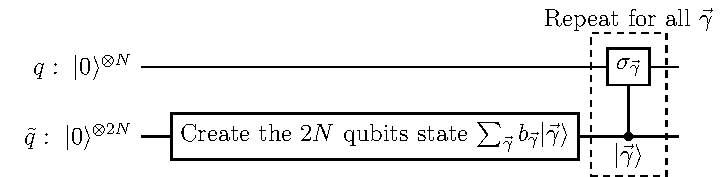
\includegraphics{images/circuito_general.pdf}
\caption{{\bf Circuit for an $N$-qubit
Pauli channel on $N$ qubits.}
The circuit creates the state $\sum_{\vec{\gamma}} b_{\vec{\gamma}}|\vec{\gamma}\rangle$ 
on the $2N$ ancilla qubits denoted by $\tilde{q}$. }
\label{fig: circuit-pauli}
\end{figure} % }}}

The first part of the circuit involves the creation of the state
\begin{eqnarray}
\label{eq: state}
\text{Ancilla state =} 
\sum_{\vec{\gamma}} b_{\vec{\gamma}} |\vec{\gamma} \rangle
\end{eqnarray}
on the ancilla qubits, where $b_{\vec{\gamma}}$ are numbers such that $
|b_{\vec{\gamma}}|^2 = k_{\vec{\gamma}}$ and
the $2N$-qubit state $|\vec{\gamma}\rangle$ is defined as $|\gamma_1\rangle
\cdots |\gamma_N\rangle$.
% \cpnote{La primera frase es cierta, pero no le veo el sentido acá. Trata de reformular el parrafo 
% de nuevo. Croe que el ``This means'' definitivamente no va y es el que le da un sentido ``raro''. 
% Itera (quizá solo quitando esas dos palabras)} \tbnote{Concuerdo, quité eso.}
When measured in the computational basis, the state given in \eref{eq: state}
collapses to $|\vec{\gamma}\rangle$ with a 
probability $|b_{\vec{\gamma}}|^2 = k_{\vec\gamma}$. 
The circuit in \fref{fig: circuit-pauli} uses this fact
to apply $\sigma_{\vec{\gamma}}$ on the main qubits
with a probability $k_{\vec\gamma}$ by using controlled operations 
conditioned on the state of the system being $|\vec{\gamma}\rangle$,
just as the Pauli channel is supposed to do.  
% 
% that apply $\sigma_{\vec{\gamma}}$ to the main qubits
% only if the ancilla qubits are in the state $|\vec{\gamma}\rangle$.
% 
% Therefore, the circuit from \fref{fig: circuit-pauli} 
% applies each operation $\sigma_{\vec{\gamma}}$ to the principal qubits 
% with a probability $k_{\vec{\gamma}}$, 
% just as a Pauli channel is supposed to do.  

\cpnote{Evaluar si al final ponemos algo al respecto de este comentario}
\cpnote{Del circuito, parece ue las fases de las bs gammas no omportan mucho (o nada). 
Esa libertad la hemos considerado? De alguna manera colapsan curvas de las que
hemos visto?} \tbnote{Sí, es una libertad que se tiene y he considerado y significa que hay muchas elecciones de $b_{\gamma}$ para un mismo canal.
Es una de las varias cosas que complicaba determinar uno a uno qué canales se pueden hacer.}


%}}}
\subsection{Simulation for one-qubit Pauli channels} % {{{
\label{subsec: Simulation for one-qubit Pauli channels}

For the particular case of a Pauli channel on one qubit, the circuit that
simulates it can be constructed as in \fref{fig: circuit-pauli-1},
which is a special case of \fref{fig: circuit-pauli}
but with all details  explicitly shown.
In said figure, the ancilla state
of \eref{eq: state} can be taken to be
$\sqrt{k_{00}} |00\rangle + \sqrt{k_{01}} |01\rangle + \sqrt{k_{10}} 
|10\rangle + \sqrt{k_{11}}|11\rangle$
and it is created on the ancilla qubits with the help of three rotations of angles:
\begin{subequations}
\begin{eqnarray}
\theta_0 &= &\arctan(\sqrt{k_{01}/k_{00}}) -
\arctan(\sqrt{k_{11}/k_{10}}),
\label{eq:angle1} \\ 
\theta_1 &= &2 \arccos(\sqrt{k_{00} +
k_{01}}),
\label{eq:angle2} \\
\theta_2 &= &\arctan(\sqrt{k_{01}/k_{00}}) +
\arctan(\sqrt{k_{11}/k_{10}}).
\label{eq:angle3}
\end{eqnarray}
\label{eq:angle}
\end{subequations}
\cpnote{Quisiera ver las ecuaciones sin la teheta despejada. Por ejemplo la de theta 1
es $\cos^2 (\theta_1/2) = k00 + k01$ bueno mas bonita, pero asi. Luego las de tehta0 y theta2 
quizá tambien sean sencillas. Las quiero ver!!!}
\tbnote{Ah, ya entiendo. Las única forma que veo de escribirlas es:
\begin{align*}
\tan \theta_0 = \dfrac{\sqrt{k_{01}/k_{00}} - \sqrt{k_{11}/k_{10}}}{1+\sqrt{\dfrac{k_{01}k_{11}}{k_{00}k_{10}}}} \\
\tan \theta_2 = \dfrac{\sqrt{k_{01}/k_{00}} + \sqrt{k_{11}/k_{10}}}{1-\sqrt{\dfrac{k_{01}k_{11}}{k_{00}k_{10}}}}
\end{align*}
No veo cómo escribir ecuaciones de las thetas no despejadas que sean sencillas.
}



\begin{figure} % {{{
\centering
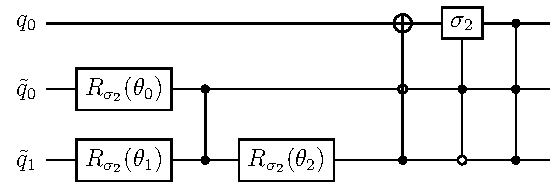
\includegraphics{images/circuito_unqubit.pdf}
\caption{
% \cpnote{ No me gusta que esté tan cargado de ecuaciones el caption. Metelas en
% el lugar apropiado en el texto} \tbnote{Lo pasé al texto}
{\bf One qubit Pauli channel circuit.} Circuit for a one-qubit Pauli channel,
which is a particular case of \fref{fig: circuit-pauli}.  Here we have two
ancilla qubits and we use three rotations
of angles given by \eref{eq:angle} to create the Ancilla State of
of \eref{eq: state} for the two ancilla qubits.
\cpnote{Creo qeu este seria el estado ecuacion 14, pero como qeuno está limpio. 
Creo quepodemos nombrar ese estado y luego referirnos acá por el nobmre y la referencia 
a la ecuación.} \tbnote{Ya}
}
\label{fig: circuit-pauli-1} 
\end{figure} % }}}


We took a sample of one-qubit Pauli channels and
used the ibmq-lima quantum computer that IBM has available~\cite{Qiskit}
to simulate them. For each of these channels, we used quantum process
tomography~\cite{Qiskit, Chuang:1996} to obtain the 
operator $\xi_I$ corresponding to the implementation of the
circuit.  Then, we compared this operator with the ideal 
channel $\xi_T$  we
wanted to implement.  


% \cpnote{Toca rediseñar este parrafo mejor. La figura que al final nos interesa
% es la $f$, pero no se menciona acá. Toca como que hacer que el párrafo gire
% alrededor de ella. }

% \tbnote{Rediseño párrafo anterior: }
% {\color{orange}  
We took a sample of one-qubit Pauli channels
and evaluated their implementation on IBM's
ibmq-lima quantum computer~\cite{Qiskit},
as shown in \fref{fig:fids}. 
For each of the channels sampled, we used 
quantum process tomography~\cite{Qiskit, Chuang:1996} to obtain the 
operator $\xi_I$ corresponding to the implementation of the
circuit in the quantum computer. 
Then, we compared $\xi_I$ with the theoretical 
operator $\xi_T$ of the Pauli channel we wanted to implement.
To see how close the operators $\xi_I$ and 
$\xi_T$ are, we shall use the
diamond distance~\cite{Aharonov,Wilde}, which is defined by
\begin{equation}
||\xi_I - \xi_T ||_{\diamond}  = \max_{\rho} || (\xi_I \otimes I) \rho - (\xi_T \otimes I) \rho ||_1,
\end{equation}
with $I$ the identity map,
$|| \cdot ||_1$ the trace norm and the maximization
done over all density matrices $\rho$.
The calculation of this norm is done using the semi-definite program from reference \cite{Watrous}.
When the two channels are the same,
the diamond distance has a value of $0$, while in the case that the channels
are completely distingushable, the distance reaches its maximum value of $2$~\cite{Benenti}.
For the analysis done in \fref{fig:fids}, we define a sort of ``diamond fidelity'' as: 
\begin{equation}
f = 1 - \dfrac{1}{2} ||\varepsilon_I - \varepsilon_T ||_{\diamond},
\label{eq:diamond-fid}
\end{equation}
which ranges from $0$, when the channels have a maximum distance, to  $1$,
when they are exactly equal.

% \cpnote{hummm ejemplo al menos para nosotros.} 
% \tbnote{Un ejemplo que comprobé es considerar el canal que aplica $\sigma_x$ y 
% el que aplica $\sigma_z$ y tienen $p_{\succ}=1$.
% De hecho, al tomar dos canales que consistan en aplicar $\sigma_i$ y $\sigma_j$ 
% (para $i\neq j$), se cumple esto.
% También quería ejemplos no unitarios, pero no encontré.}

Finally, using the representation of Pauli channels in a tetrahedron as
in \eref{eq: conditions-tetrahedron},
we show in \fref{fig:fids} the diamond fidelity defined by \eref{eq:diamond-fid} for the channels
analyzed. 
We can see that channels close to the 
completely depolarizing
channel (that is close to the center of the tetrahedron)
have a high $f$, while those 
close to unitary channels have much lower $f$.
This means that channels closer to the 
completely depolarizing channel are simulated better on the quantum computers.
This is reasonable because quantum computers are prone to errors
that depolarize qubits, which isn't very problematic
when trying to simulate depolarization but it is 
when simulating unitary processes. \cpnote{Tambien creo qeu debemos comentar que nuestra 
simulación para operaciones unitarias no es optima, porque usamos un monton de compuertas 
y además operaciones doblemente controladas.}
\tbnote{Algo como: }
{\color{orange} Moreover, the algorithm of \fref{fig: circuit-pauli-1} is not optimal for unitary channels 
(that is, the channels corresponding to the vertices of the tetrahedron). 
These straightforward channels could be accomplished more efficiently by simply applying the corresponding Pauli operation directly. Nevertheless, due to its general design to accommodate any Pauli channel, the algorithm employs numerous quantum gates even in such scenarios.}
\cpnote{Siento qeu aun falta algo de análisis pero lo dejamos para cuando tengamos mas
figuras y mas inspiracion}
\tbnote{Va}

\begin{figure} % {{{
\centering
\begin{subfigure}{0.9\textwidth}
\begin{subfigure}{.666\textwidth}
\centering
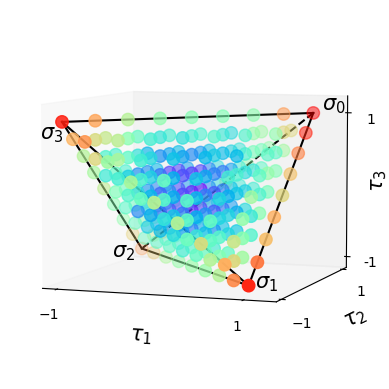
\includegraphics[width=.95\columnwidth]{images/tetra-def.png}
\end{subfigure}%
\begin{subfigure}{.333\textwidth}
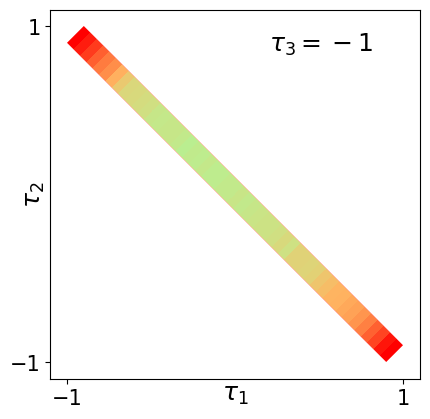
\includegraphics[width=.95\columnwidth]{images/corte1-2.png} \\
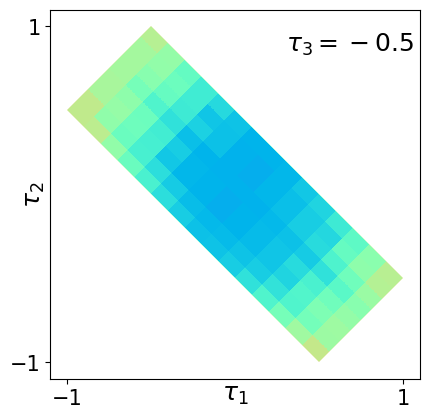
\includegraphics[width=.95\columnwidth]{images/corte2-2.png} \\
\end{subfigure}
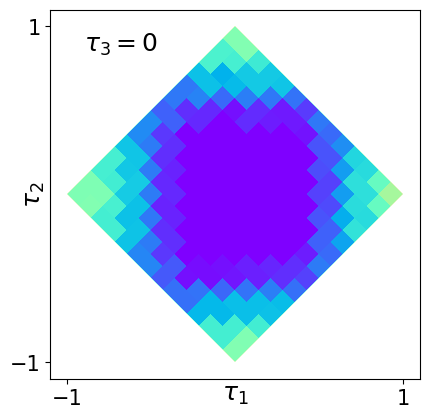
\includegraphics[width=.322\columnwidth]{images/corte3-2.png}
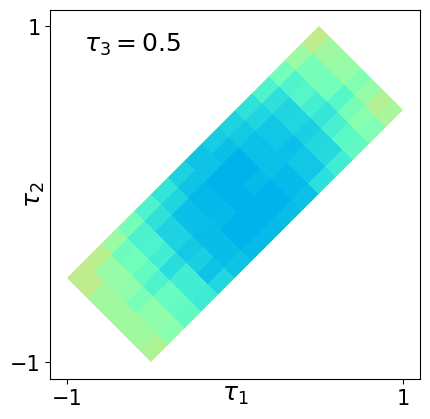
\includegraphics[width=.322\columnwidth]{images/corte4-2.png}
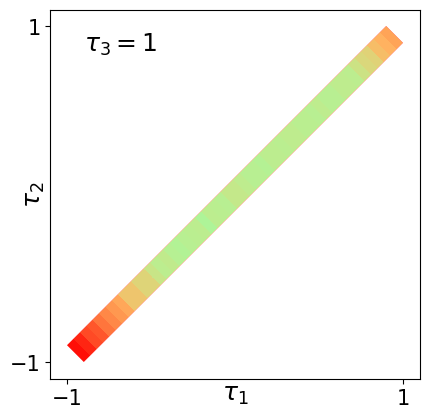
\includegraphics[width=.322\columnwidth]{images/corte5-2.png}
\end{subfigure}%
\begin{subfigure}{0.1\textwidth}
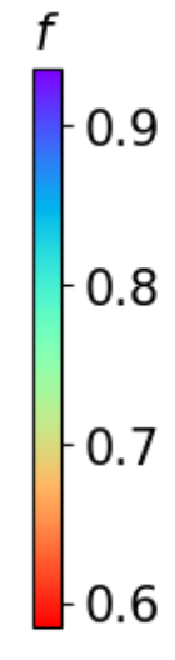
\includegraphics[width=.8\columnwidth]{images/col-2.png} \\ [2ex]
\end{subfigure}
\caption{Results of the diamond fidelities as defined in \eref{eq:diamond-fid}
for a sample of Pauli channels in the tetrahedron.  Notice that channels close
to the center of the tetrahedron have high fidelities, while those close to the
borders do not.  Moreover, we show the results for cuts of the tetrahedron at
different values of $\tau_3$.}
\label{fig:fids}
\end{figure} % }}}





% }}}
% }}}
\section{One Parameter Circuits} % {{{
\label{sec: 1PR Circuits}


Just as Pauli channels, Pauli dynamical maps can be implemented using the circuit
of \fref{fig: circuit-pauli}. However, there is one difference: 
the state to be created on the ancilla qubits now 
depends on a parameter $p$, and it is represented by the expression:
\begin{eqnarray}
\label{eq: parametrized state}
\sum_{\vec{\gamma}} b_{\vec{\gamma}}(p) |\vec{\gamma}\rangle.
\end{eqnarray}
Thus, we temporarily shift our focus from Pauli
channels and dynamical maps to the general problem of 
creating a circuit to generate a curve of
states like the one described in \eref{eq: parametrized state}.

In general, producing this curve of states for $N$ qubits will require
many rotations parametrized by $p$,
such as the three rotations used for the ancilla
qubits in \fref{fig: circuit-pauli-1}.
However, it would be preferable to achieve the same effect using only one parametrized rotation. 
This would allow us to interpret said rotation 
as a knob that smoothly traverses the curve of states.
Consequently, we are faced with the question of which curves of states, 
such as the one described in \eref{eq: parametrized state}, 
can be produced using just a single parametrized rotation. 
To clarify this, we provide the following definition 
for a circuit with one parametrized rotation.

\begin{definition}{\textbf{1-Parameter Rotation Circuit:}}
A 1-Parameter Rotation (1PR) circuit is a parametrized quantum
circuit that includes only one gate dependent on a parameter $p$.
Moreover, the parametrized gate is a one-qubit rotation about any axis,
whether controlled or not.
\end{definition}

Based on this definition, we aim to determine which curves of 
states can be generated using 1PR circuits. 
To accomplish this, we begin by proving that all 1PR circuits have 
the form depicted in \fref{fig:1PR-circuit},
where the parametrized rotation is around $\sigma_3$ and
is applied to the last qubit.

\begin{figure} % {{{
\centering
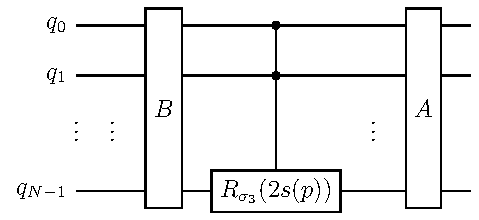
\includegraphics{images/OPR-circuit.pdf}
\caption{\textbf{General form of a 1PR circuit}.
Any 1PR circuit can be transformed into this form,
where the rotation on the last qubit
can be controlled or not by any of the other qubits.
$A$ and $B$
are $N$-qubit gates that do not depend on the parameter $p$ and
$s= s(p)$ is a function of the parameter.
}
\label{fig:1PR-circuit}
\end{figure} % }}}

\begin{theorem}
An $N-$qubit 1PR circuit can always be transformed 
into the form shown in \fref{fig:1PR-circuit}.
\end{theorem}
\textbf{Proof:} 
First, we observe that according to the
definition, a 1PR circuit always consists of an operation $B$ followed 
by the parametrized rotation and then another operation $A$, 
where $A$ and $B$ are not parametrized.

Next, we note that it is not necessary to consider rotations about an arbitrary axis,
as a rotation about any axis $\hat{n}$ parameterized by $p$
can be transformed into a rotation about $\sigma_3$ without introducing 
gates that depend on $p$. To see this, consider the rotation $R_{\hat{n}}(2s)$, where $2s$ 
is a function of $p$ (the factor of 2 is for convenience later on) 
and $\hat{n} = (n_1,n_2,n_3)$ represents the rotation axis. 
We can express $\hat{n}$ as $(\sin \theta \cos \phi, \sin \theta \sin \phi, \cos \theta)$, 
where $\theta$ and $\phi$ are fixed angles dependent on $\hat{n}$. 
The rotation can then be rewritten as follows:
\begin{eqnarray}
R_{\hat{n}}(2s) = R_{\sigma_3}(\phi) R_{\sigma_2}(\theta) R_{\sigma_3}(2s) R_{\sigma_2}(-\theta) R_{\sigma_3}(-\phi).
\end{eqnarray}
Since the angles $\theta$ and $\phi$ do not depend on the parameter $p$,
any 1PR circuit can be transformed into a circuit where the parametrized
 rotation is around $\sigma_3$ instead of an arbitrary axis. 
Moreover, without loss of generality, we can choose the last qubit as the
target qubit for the rotation, since if it weren't, we could use
swap gates to move the rotation
to the first qubit without adding gates
that depend on $p$. 

Therefore, a 1PR circuit can be transformed such
that the rotation is around $\sigma_3$ and is applied to the last qubit 
(possibly controlled by other qubits), 
resulting in the form depicted in \fref{fig:1PR-circuit}. 
$\blacksquare$ \\
$\;$\\

With the aid of this theorem, we can now determine the curves
of states of $N$ qubits that can be generated using a 1PR circuit. 
This result is stated in the following theorem.

\begin{theorem}
Consider a 1PR circuit of $N$ qubits
and denote by $U$ the operator it implements on this system. 
Then, for every $j \in \{0, 1, \cdots, 2^N-1\}$, 
we have that:
\begin{align*}
U|j\rangle = e^{is} |a^j\rangle + e^{-is} |b^j\rangle + |c^j\rangle
\end{align*}
with $|a^j\rangle ,|b^j\rangle, |c^j\rangle$ orthogonal states and $|a^j|^2 + |b^j|^2 + |c^j|^2 = 1$.
\end{theorem}
\textbf{Proof:} 
\cpnote{Sugiero cambiar la a gargoleada por una a con gorro o con tilde. No se 
usa asi cambiar de fuente.} \tbnote{Va, listo}
We can conclude from theorem 1 that $U=ARB$,
where $A$ and $B$ are unitary matrices and $R$ is a $\sigma_3$ rotation of angle $2s$
applied to the last qubit and controlled by some of the other ones. 

First, applying $B$ to $|j\rangle$ results in $B|j\rangle = B_{0,j} |0\rangle + B_{1,j} |1 \rangle + \cdots + B_{2^n-1,j}|2^n-1\rangle$,
with $B_{i,j}$ the entries of matrix $B$.
This can be rewritten by separating last qubit from the other $N-1$:
\begin{equation}
B|j\rangle = \sum_{k=0}^{2^{N-1}-1} \left( B_{2k,j} |k\rangle|0\rangle  + B_{2k+1,j} |k \rangle |1\rangle  \right).
\end{equation}
After the operator $B$, the circuit applies the  controlled rotation $R$.
To simplify the analysis, we separate the states of
the first $N-1$ qubits into those that fulfill the control conditions of the rotation
(which we denote as the set $\mathcal{C}$)
and those that do not, and write it as
\begin{align}
B|j\rangle = 
   \sum_{k \in \mathcal{C}} \left( B_{2k,j} |k\rangle|0\rangle 
                                     + B_{2k+1,j} |k \rangle |1\rangle  \right) 
   + \sum_{k \not\in \mathcal{C}} \left( B_{2k,j} |k\rangle|0\rangle  
                                      + B_{2k+1,j} |k \rangle |1\rangle  \right).
\end{align}

\cpnote{Separo el parrafo par auqe cada matriz tenga como su propio espacio.} \tbnote{Va, excelente.}
Then, the rotation $R$ will only affect the states on the first sum (since they fulfill the control conditions)
and not the others. Therefore,  
remembering that a $\sigma_3$ rotation acts by adding a phase $e^{-is}$ to $|0\rangle$
and a phase $e^{is}$ to $|1\rangle$, we have that,
% \begin{small}
% \begin{eqnarray}
% &e^{-is} \sum_{k \in \mathcal{C}} B_{2k,j} |k\rangle |0\rangle + e^{is} \sum_{k \in \mathcal{C}} B_{2k+1,j} |k\rangle |1 \rangle 
% + \sum_{k \not\in \mathcal{C}} \left( B_{2k,j} |k\rangle |0\rangle + B_{2k+1} |k\rangle |j \rangle \right)\\
% & \qquad = e^{-is} \vec{b'}_j + e^{is} \vec{a'}_j + \vec{c'}_j,
% \end{eqnarray}
% \end{small}
% test
\begin{align}
RB|j\rangle& = e^{-is} \sum_{k \in \mathcal{C}} B_{2k,j} |k\rangle |0\rangle + e^{is} \sum_{k \in \mathcal{C}} B_{2k+1,j} |k\rangle |1\rangle 
+ \sum_{k \not\in \mathcal{C}} \left( B_{2k,j} |k\rangle|0\rangle  + B_{2k+1,j} |k \rangle |1\rangle  \right) \nonumber \\
& = e^{-is} |\tilde{b}^{j}\rangle + e^{is} |\tilde{a}^j\rangle + |\tilde{c}^j\rangle
\end{align}
where we defined
\begin{align*}
|\tilde{a}^j \rangle &= \sum_{k \in \mathcal{C}} B_{2k,j}|k\rangle|0\rangle,\\
|\tilde{b}^j\rangle &= \sum_{k \in \mathcal{C}} B_{2k+1,j} |k\rangle |0 \rangle,\\
|\tilde{c}^j\rangle &= \sum_{k \not\in \mathcal{C}}\left( B_{2k,j} |k\rangle|0\rangle+ B_{2k+1,j} |k \rangle |1\rangle  \right).
\end{align*}
\cpnote{Acá puedes usar align. Creo que es mucho para dejarlas en el texto. Recuerda la puntuacion. 
Me está gustando mucho la explicacion. Simple y clara. }
\tbnote{Listo.}
These states are clearly orthogonal because they are each linear combinations of different 
orthogonal states of the computational basis. 
Moreover, they satisfy  $|\tilde{a}^j|^2 + |\tilde{b}^j|^2 + |\tilde{c}^j|^2 = 1$ because this quantity is the squared norm of the $j$th column of $B$, 
which is unitary.

Finally, after having applied the rotation, the circuit applies gate $A$, 
so that the result is given by:
\begin{eqnarray}
U|j\rangle = ARB|j\rangle = e^{-is} A |\tilde{a}^j\rangle + e^{is} A |\tilde{b}^j\rangle + A |\tilde{c}^j\rangle = e^{-is} |a^j\rangle + e^{is} |b^j\rangle + |c^j\rangle,
\end{eqnarray}
where $|a^j\rangle = A |\tilde{a}^j\rangle, |b^j\rangle = A |\tilde{b}^j\rangle, |c^j\rangle = A |\tilde{c}^j\rangle$ are still orthogonal
states that satisfy $|a|^2 + |b|^2 + |c|^2 = 1$ because $A$ is unitary. $\blacksquare$  \\
 $\;$ \\

\cpnote{Acá voy}
 
This theorem implies that starting from the state $|0\rangle$ (or any 
other starting state),
the only curves of states we could expect to create
with a 1PR circuit are those of the form $U|0\rangle$, that is, curves such as:
\begin{equation}
|\eta(p)\rangle = |c\rangle + e^{is}|a\rangle + e^{-is} |b\rangle,
\label{eq:curve-states}
\end{equation}
with 
\begin{equation}
|a|^2 + |b|^2 + |c|^2 = 1  \; \text{and} \; |a\rangle, |b\rangle, |c\rangle \; \text{orthogonal states},
\label{eq:conditions-vecs}
\end{equation}
and $s = s(p)$ a function of $p$.
Furthermore, given a curve of states as the one in
\eref{eq:curve-states}, we can always construct a 1PR circuit to create it.
One way of doing it, is to use the circuit of \fref{fig:1PR-circuit}, setting the parametrized
rotation $R$ on the last qubit to be controlled by all the other qubits
and defining the operators $A$ and $B$ by:
\begin{align*}
&B|0\rangle = |a| |2^{N}-1 \rangle + |b| |2^{N}-2\rangle + |c| |2^N-3\rangle, \\
&A|2^N-1 \rangle = \frac{1}{|a|} |a\rangle,\; A|2^{N}-2\rangle = \frac{1}{|b|}|b\rangle, \; A|2^{N}-3\rangle = \frac{1}{|c|}|c\rangle.
\end{align*}
The rest of the operators $A$ and $B$ can be
defined arbitrarily in any way such that they are unitary.
Then, starting from the initial state $|0\rangle$
and applying the circuit  of \fref{fig:1PR-circuit}, 
some direct calculations lead us  to 
the resulting curve of states
of \eref{eq:curve-states}.
To see it, notice that rewriting the expression of  $B|0\rangle$ by separating the
first $N-1$ qubits from the last one,
we have that $$B|0\rangle = |a| |2^{N-1}-1\rangle |1\rangle + |b| |2^{N-1}-1\rangle |0\rangle + |c| |2^{N-1}-2\rangle |1\rangle.$$
Then, since the parametrized rotation $R$ is controlled by all the first $N-1$ qubits, it only applies
to the first two terms of $B|0\rangle$ 
and gives as a result
$$
RB|0\rangle =|a| e^{is} |2^{N-1}-1\rangle |1\rangle + |b| e^{-is} |2^{N-1}-1\rangle |0\rangle + |c| |2^{N-1}-2\rangle |1\rangle.
$$
Finally, applying $A$ as defined above to this state leads to the desired result.
 
%Therefore, from this theorem we conclude that
%the kind of curves of states that can be created
%using a 1PR circuit are always of the form
%\begin{align*}
%|b(p)\rangle= e^{is} \vec{a} + e^{-is} \vec{b} + \vec{c},
%\end{align*}
%where $s$ is a function of $p$, $\vec{a},\vec{b},\vec{c}$ are orthogonal vectors and
%$|\vec{a}|^2+  |\vec{b}|^2 + |\vec{c}|^2 = 1$.
%%\textbf{Puntos:}
%\begin{itemize}
%\item As said before, to implement a Pauli dynamical map, 
%we need to create the parametrized $2n$-qubit state 
%$\sum_{\vec{\gamma}} b_{\vec{\gamma}}(p) |\vec{\gamma}\rangle$ on the ancilla qubits.
%\item However, creating this state will in general require many rotations parametrized by $p$. 
%For example, for the case of a Pauli dynamical map on 1 qubit, 
%the parametrized state of the $2$ ancilla qubits in general requires $3$ parametrized rotations and can be constructed as follows: (poner circuito).\\
%In general, to create a parametrized state on $2n$ ancilla qubits will require
%$2n-1$ rotations parametrized by $p$.
%\item How can we reduce the amount of parametrized rotations used?
%\item \textbf{1PR Circuit:} Define an 1PR circuit (a circuit with one parametrized rotation)
%\item \textbf{Theorem about 1PR circuits:} \textit{An 1PR circuit on $n$ qubits with parameter $p$ always has an operator of the form:}
%\begin{eqnarray}
%U = (\vec{v}_0| \vec{v}_1| \cdots| \vec{v}_{2^n-1})
%\end{eqnarray}
%\textit{where $s = s(p)$ and the column vectors are $\vec{v}_j = e^{is} \vec{a}_j + e^{-is} \vec{b}_j + \vec{c}_j$, with $\vec{a}_j, \vec{b}_j, \vec{c}_j$ orthogonal vectors and $|\vec{a}_j|^2 + |\vec{b}_j|^2 + |\vec{c}_j|^2 = 1$.}
%\item \textbf{Proof:} La prueba está dentro de las ``Cosas-Escritas-Antes'', 
%aunque se puede y debe achicar bastante.
%\end{itemize}
% }}}

\section{1PR circuit for a Pauli map} % {{{
\label{sec: 1PR circuit for a Pauli map}


We can now use the previous results to conclude directly which Pauli dynamical maps
can be implemented with a 1PR circuit.
Given this condition, the curve of states of \eref{eq: parametrized state}  needed 
to implement the map
has to be constructed with only one parametrized rotation. 
Therefore, the results of the last section imply that the the map
\begin{eqnarray}
\varepsilon_p(\rho) = \sum_{\vec{\gamma}} k_{\vec{\gamma}}(p) \sigma_{\vec{\gamma}} \rho \sigma_{\vec{\gamma}},
\end{eqnarray}
can be implemented  if there are numbers $\beta_{\vec{\gamma}}(p)$ such that $|\beta_{\vec{\gamma}}(p)|^2 = k_{\vec{\gamma}}(p)$ and
\begin{eqnarray}
\label{eq:vec}
\sum_{\vec{\gamma}} \beta_{\vec{\gamma}}(p) |\vec{\gamma}\rangle = |c\rangle +  e^{is} |a\rangle + e^{-is}|b\rangle,
\end{eqnarray}
where $|a\rangle,|b\rangle,|c\rangle$ are orthogonal states in  
and $|a|^2+  |b|^2 + |c|^2= 1$.

For the particular case of one qubit,
we can show some examples of Pauli dynamical maps
implementable with a 1PR circuit, which are plotted
in \fref{fig:curves1}.


\begin{figure}
\captionsetup[subfigure]{justification=centering}
\centering
\begin{subfigure}{.45\textwidth}
  \centering
  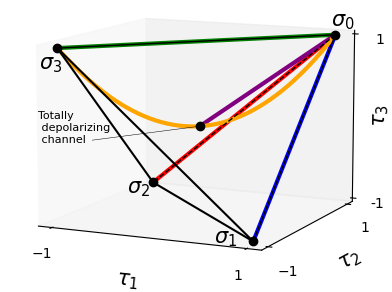
\includegraphics[width=.9\linewidth]{images/curvas.png}
   \caption{}
  \label{fig:curves1}
\end{subfigure}%
\begin{subfigure}{.45\textwidth}
  \centering
  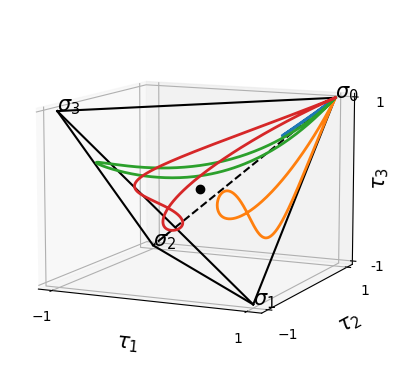
\includegraphics[width=.9\linewidth]{images/curvas-azar.png}
  \caption{}
  \label{fig:curves2}
\end{subfigure}
\caption{{\bf Some Pauli dynamical maps that can be implemented with a 1PR circuit.}
The curves painted in these tetrahedrons
represent Pauli dynamical maps that can be implemented with 1PR circuits.
(a) shows the dynamical maps mentioned in the main 
text, which are: depolarizing (purple), bit flip (blue),
phase flip (green), bit-phase flip (red)
and parabolic (orange).
(b) shows dynamical maps selected at random that can be implemented with 1PR 
circuits.}
\label{fig:curves}
\end{figure}


\begin{itemize}
\item \textbf{Bit flip map:} 
This dynamical map is defined as
\begin{align*}
\varepsilon_p(\rho) = (1-p)\rho + p\sigma_1 \rho \sigma_1,
\end{align*}
for $p \in [0,1]$. 
Therefore, the curve of states $|\beta(p)\rangle$ needed on the ancilla
qubits is such that 
$|\beta_0(p)|^2= (1-p)^2$, $|\beta_1(p)|^2 = p$, $|\beta_2(p)|^2 = |\beta_3(p)|^2 = 0$.
In particular, if we take the $\beta_j$ to be real,
we need to create the curve of states:
\begin{align*}
|\beta(p)\rangle = \sqrt{1-p} |0\rangle +\sqrt{p} |1\rangle.
\end{align*}
This can be rewritten as
\begin{align*}
|\beta(p) \rangle = e^{is}  \left(\frac{1}{2} |0\rangle - \dfrac{i}{2} |1\rangle \right) + e^{-is} \left( \frac{1}{2} |0\rangle + \frac{i}{2} |1\rangle \right),
\end{align*}
with $s= \arcsin(\sqrt{p})$.
Therefore, we can see that the curve satisfies the conditions of  \eref{eq:conditions-vecs} 
and it can be created with a 1PR circuit.
The exact same thing can be done
for the phase flip and bit phase flip dynamical maps by
changing $\sigma_1$ to
$\sigma_3$ and $\sigma_2$ respectively.

\item \textbf{Depolarizing:} This dynamical map is given by
\begin{align*}
\varepsilon_p(\rho) = (1-3p/4) \rho + (p/4) \sigma_1 \rho \sigma_1 + (p/4) \sigma_2 \rho \sigma_2 + (p/4) \sigma_3 \rho \sigma_3,
\end{align*}
with $p \in [0,1]$. 
Then, taking the $\beta_j$ to be real,
the curve of states needed to create on the ancilla qubits is
\begin{align*}
|\beta(p) \rangle = \sqrt{1-3p/4} |0\rangle + \sqrt{p/4} |1\rangle + \sqrt{p/4} |2 \rangle  + \sqrt{p/4} |3\rangle.
\end{align*}
This state can be rewritten as:
\begin{align*}
|\beta(p)\rangle =& \; e^{is} \left( \dfrac{1}{2} |0\rangle - \dfrac{i}{2\sqrt{3}} |1\rangle - \dfrac{i}{2\sqrt{3}} |2 \rangle - \dfrac{i}{2\sqrt{3}} |3\rangle \right) \\
& + e^{-is} \left( \dfrac{1}{2} |0\rangle + \dfrac{i}{2\sqrt{3}} |1\rangle + \dfrac{i}{2\sqrt{3}} |2\rangle + \dfrac{i}{2\sqrt{3}} |3 \rangle \right),
\end{align*}
with $s = \arcsin(\sqrt{3p/4})$.
We can see that this curve satisfies the conditions of \eref{eq:conditions-vecs}, meaning that it can be created with a 
1PR circuit.

\item \textbf{Parabolic dynamical map:} Finally, we define the parabolic dynamical map as:
\begin{eqnarray}
\epsilon(\rho) = \dfrac{1}{4} (1-p)^2  \rho + \dfrac{1}{4} (1-p^2) \sigma_1 \rho \sigma_1 + \dfrac{1}{4} (1-p^2) \sigma_2 \rho \sigma_2 + \dfrac{1}{4} (1+p)^2 \sigma_3 \rho \sigma_3 ,
\end{eqnarray}
with $p \in [-1,1]$. 
If we take the $\beta_j$ to be real,
we need to create the curve of states:
\begin{eqnarray}
|\beta(p)\rangle = \dfrac{1}{2} (1-p) |0\rangle + \dfrac{1}{2} \sqrt{1-p^2} |1\rangle +  \dfrac{1}{2} \sqrt{1-p^2} |2\rangle +  \dfrac{1}{2}(1+p) |3\rangle.
\end{eqnarray}
This can be rewritten as
\begin{align*}
|\beta(p)\rangle =&\; \left( \dfrac{1}{2}|0\rangle + \dfrac{1}{2} |3\rangle \right) + e^{is} \left( \dfrac{i}{4}|0\rangle + \dfrac{1}{4} |1\rangle + \dfrac{1}{4} |2\rangle - \dfrac{i}{4} |3\rangle \right) \\
& + e^{-is}  \left( \dfrac{-i}{4} |0\rangle + \dfrac{1}{4} |1\rangle + \dfrac{1}{4} |2\rangle + \dfrac{i}{4} |3\rangle \right),
\end{align*}
with $s = \arcsin(p)$, so that
this map fulfills the conditions of  \eref{eq:conditions-vecs}.
\end{itemize}

Furthermore, we can construct other examples of 
Pauli dynamical maps such that they
can be implemented with a 1PR circuit.
To do it, we only need to choose the three states $|a\rangle, |b\rangle, |c\rangle$
that satisfy the conditions of  \eref{eq:conditions-vecs}.
For example, this can be done systematically for the case of curves of states of two qubits
(that is, for Pauli dynamical maps of one qubit)
with the following procedure:
\begin{itemize}
\item[1.] We first choose the norms $|a|, |b|, |c|$
such that $|a|^2 + |b|^2 + |c|^2 = 1$. 
This can be done by selecting two angles
$\mu \in [0, \pi/2] , \nu \in [0,\pi/2]$ and defining:
\begin{align*}
|a| = \sin \nu \cos \mu, \; |b| = \sin \nu \sin \mu , \; |c| = \cos \nu.
\end{align*}
\item[2.] We define $|a'\rangle = |a| |0\rangle$, $|b'\rangle = |b| |1\rangle,$ $|c'\rangle = |c| |2\rangle$.
\item[3.] Finally, we choose a unitary matrix $V$
and use it to define the states $|a\rangle = V |a'\rangle, |b\rangle = V |b'\rangle, |c\rangle = V |c'\rangle$.
This way, since the primed states are orthogonal and their squared norms add up to one,
so do the unprimed states and therefore 
fulfill the conditions of  \eref{eq:conditions-vecs}. 
\end{itemize}

Following this procedure for random
angles and unitary matrices $V$, 
we plot four Pauli dynamical maps 
that can be implemented with a 1PR circuit in \fref{fig:curves2}.
These maps where constructed with the additional condition
of the map passing through the identity channel.
To do that, we ensure that the vectors also satisfy
$|a\rangle + |b\rangle + |c\rangle = e^{i \theta}|0\rangle$ with $\theta$ an arbitrary
real number.
This way, when $s = 0$ in \eref{eq:vec}, the constructed state
is $e^{i \theta}|0\rangle$, which
corresponds with the identity channel.

To fulfill this additional condition,  we restrict the first row of
$V$ writen as a matrix in 
the computational basis to be $e^{i\theta} (|\vec{a}|, |\vec{b}|, |\vec{c}|,0)$. 
That way, 
\begin{align*}
|a\rangle + |b\rangle + |c\rangle = V (|a'\rangle + |b'\rangle + |c'\rangle ) = V(|\vec{a}|, |\vec{b}|, |\vec{c}|,0)^T = (e^{i\theta},0,0,0)^T.
\end{align*}
The last step is because the first entry of $V(|\vec{a}|, |\vec{b}|, |\vec{c}|,0)^T$
is obtained by calculating the dot product of the first row of $V$ with $(|\vec{a}|, |\vec{b}|, |\vec{c}|,0)^T$, which gives
$e^{i\theta}$. 
Furthermore, the other entries have to be $0$,
since otherwise the norm of the result would be greater than
$1$ but $V$ is unitary and therefore preserves the norm.





\section{Conclusion} % {{{
\tbnote{Poner luego}
% }}}
\section{Supporting information} % {{{

\tbnote{Ver qué se debe de poner aquí según el template y también arreglar las imágenes de acuerdo a él.}
% Include only the SI item label in the paragraph heading. Use the \nameref{label} command to cite SI items in the text.
\paragraph*{S1 Fig.}
\label{S1_Fig}
{\bf Bold the title sentence.} Add descriptive text after the title of the item (optional).

\paragraph*{S2 Fig.}
\label{S2_Fig}
{\bf Lorem ipsum.} Maecenas convallis mauris sit amet sem ultrices gravida. Etiam eget sapien nibh. Sed ac ipsum eget enim egestas ullamcorper nec euismod ligula. Curabitur fringilla pulvinar lectus consectetur pellentesque.

\paragraph*{S1 File.}
\label{S1_File}
{\bf Lorem ipsum.}  Maecenas convallis mauris sit amet sem ultrices gravida. Etiam eget sapien nibh. Sed ac ipsum eget enim egestas ullamcorper nec euismod ligula. Curabitur fringilla pulvinar lectus consectetur pellentesque.

\paragraph*{S1 Video.}
\label{S1_Video}
{\bf Lorem ipsum.}  Maecenas convallis mauris sit amet sem ultrices gravida. Etiam eget sapien nibh. Sed ac ipsum eget enim egestas ullamcorper nec euismod ligula. Curabitur fringilla pulvinar lectus consectetur pellentesque.

\paragraph*{S1 Appendix.}
\label{S1_Appendix}
{\bf Lorem ipsum.} Maecenas convallis mauris sit amet sem ultrices gravida. Etiam eget sapien nibh. Sed ac ipsum eget enim egestas ullamcorper nec euismod ligula. Curabitur fringilla pulvinar lectus consectetur pellentesque.

\paragraph*{S1 Table.}
\label{S1_Table}
{\bf Lorem ipsum.} Maecenas convallis mauris sit amet sem ultrices gravida. Etiam eget sapien nibh. Sed ac ipsum eget enim egestas ullamcorper nec euismod ligula. Curabitur fringilla pulvinar lectus consectetur pellentesque.
% }}}
\section{Acknowledgments} % {{{
Support by projects CONACyT 285754, 254515 and UNAM-PAPIIT IG100518, IG101421 is
acknowledged. 


\nolinenumbers

% }}}
% Biblbiografia {{{
% Either type in your references using
% \begin{thebibliography}{}
% \bibitem{}
% Text
% \end{thebibliography}
%
% or
%
% Compile your BiBTeX database using our plos2015.bst
% style file and paste the contents of your .bbl file
% here. See http://journals.plos.org/plosone/s/latex for 
% step-by-step instructions.
% 
%\begin{thebibliography}{10}
%
%\bibitem{bib1}
%Conant GC, Wolfe KH.
%\newblock {{T}urning a hobby into a job: how duplicated genes find new
%  functions}.
%\newblock Nat Rev Genet. 2008 Dec;9(12):938--950.

%\bibitem{bib2}
%Ohno S.
%\newblock Evolution by gene duplication.
%\newblock London: George Alien \& Unwin Ltd. Berlin, %Heidelberg and New York:
%  Springer-Verlag.; 1970.

%\bibitem{bib3}
%Magwire MM, Bayer F, Webster CL, Cao C, Jiggins FM.
%\newblock {{S}uccessive increases in the resistance of {D}rosophila to viral
%  infection through a transposon insertion followed by a {D}uplication}.
%\newblock PLoS Genet. 2011 Oct;7(10):e1002337.
%
%\end{thebibliography}
\tbnote{Poner la bibliografía como ellos dicen (copiarla toda aquí en lugar de ponerla en un archivo .bib)}
\textbf{References}
\bibliography{Bibliography}

% }}}
\newpage
\appendix
%\section{Resumen}
\begin{itemize}
\item In this work we study parametrized quantum circuits used to implement
quantum operations over qubit systems. 
\item Specifically, we study two types of operations: Pauli
dynamical maps and transformations of the form $e^{iHt}$ on $n$ qubits. 
\item We focus mainly on operations that can be implemented using a circuit 
with only one parametrized rotation gate (OPR Circuit). 
\item We get the conditions on these operations to be
applied with an OPR circuit:\\

\textbf{Theorem:} An OPR circuit with parameter $p$ on $n$ qubits always has an operator of the form:
\begin{eqnarray}
U  = (\vec{v}_0, \vec{v}_1, \cdots, \vec{v}_{2^n-1})
\end{eqnarray}
where $s = s(p)$ and the column vectors are $\vec{v}_j = e^{is} \vec{a}_j + e^{-is} \vec{b}_j + \vec{c}_j$, with $\vec{a}_j, \vec{b}_j, \vec{c}_j$ orthogonal vectors and $|\vec{a}_j|^2 + |\vec{b}_j|^2 + |\vec{c}_j|^2 = 1$. \\

\item We propose a circuit to simulate Pauli dynamical maps on $n$ qubits using $2n$ ancilla qubits. We find the conditions for channels that can be simulated by an OPR circuit and some examples that fulfill these conditions. 

\item We find the conditions that a matrix $H$ must have for the operation $e^{iHt}$ to be implementable with an OPR circuits: \\

 \textbf{Theorem:} An $n-$qubits operator $U = e^{iHt}$ (with $H$ time-independent) can be implemented using an OPR circuit if and only if the eigenvalues of $H$ are $-\lambda, 0, \lambda$ (for $\lambda$ a real number) and the degeneracies of $\lambda$ and $-\lambda$ are $2^j$ for some $j$ such that $0 \leq j <n$.
\item We find how to construct the OPR circuit that implements $e^{iHt}$ given the conditions of the theorem and see some examples. 

\item Finally, we implement some of these
circuits on IBM's quantum computers and obtain their fidelities.
\end{itemize}
\newpage


\section{Partes más desarrolladas}
\subsection{Resumen}
In this work we study parametrized quantum circuits used to 
implement quantum operators over qubits systems on a quantum computer. 
Specifically, we study Pauli dynamical maps and unitary transformations of the form $e^{iHt}$.
 We focus mainly on operations that can be implemented using a circuit  with only one parametrized rotation gate (OPR circuit),
 and get the conditions these operations must satisfy for 
 being applicable on an OPR circuit.
Finally, we implemented some specific examples of these circuits on IBM's quantum computers
and obtain the fidelity of this implementation.

\subsection{Introduction}
\begin{itemize}
\item 
\end{itemize}

\subsection{OPR Circuits}

\textbf{Definition, Circuit with one parametrized Gate (OPR circuit):} A quantum circuit
 that contains only one gate that depends on a parameter $p$.
Furthermore, the parametrized gate is a one qubit rotation about any axis. \\

\textbf{Property 1:} \textit{An $n$-qubit OPR circuit can always be transformed into the form of circuit \ref{fig: OPR general-A}, where $A$ and $B$ are $n$-qubit gates that don't depend on the parameter
and $s = s(p)$ is a function of the parameter.}\\

\begin{figure}[h!]
\centering
\begin{quantikz}
\lstick{$q_0$} & \qw & \gate[wires = 4,nwires=3]{B} & \ctrl{3} & \qw & \gate[wires=4,nwires=3]{A} & \qw \\
\lstick{$q_1$} & \qw &  & \ctrl{2} & \qw & & \qw \\
\vdots & \vdots & & & \vdots & \\
\lstick{$q_{n-1}$} & \qw & & \gate{R_{\sigma_3}(2s(p))} & \qw & & \qw
\end{quantikz}
\caption{Forma general de un circuito RP.}
\label{fig: OPR general-A}
\end{figure}

First of all, we notice that by definition an OPR
will always consist on some operation $B$ followed by the parametrized rotation 
and then some operation $A$, where $A$ and $B$ are not parametrized. 

Then, we notice that it isn't necessary to consider rotations
about an arbitrary axis, since a rotation about $\hat{n}$ parametrized by $p$ can
be converted into a rotation about $\sigma_3$ without the need of introducing gates that depend on $p$.
To see this, consider the rotation $R_{\hat{n}}(2s)$, where $2s$ is some function of $p$ (the $2$ is added for convenience later on) and $\hat{n} = (n_1,n_2,n_3)$ is the rotation axis,
 which can be written as $(n_1,n_2,n_3) = (\sin \theta \cos \phi , \sin \theta\sin \phi, \cos \theta)$ for some fixed angles $\phi, \theta$ dependent on $\hat{n}$. 
 Then, the rotation can be rewritten as (ref 12 de la tesis):
\begin{eqnarray}
R_{\hat{n}}(2s) = R_{\sigma_3}(\phi) R_{\sigma_2}(\theta) R_{\sigma_3}(2s) R_{\sigma_2}(-\theta) R_{\sigma_3}(-\phi).
\end{eqnarray}
Because angles $\theta, \phi$ don't depend on the parameter $p$, 
any OPR circuit can be converted into a circuit in which the parametrized rotation is around $\sigma_3$ instead of an arbitrary axis.

Furthermore, the qubit to which the rotation is applied can be selected to be the last one,
since otherwise  swap gates can be added before and after the rotation to make it act on the last qubit.

Therfore, an OPR circuit can be transformed in a way that the rotation is around $\sigma_3$ and applied on the last qubit 
(possibly controlled by other qubits), 
so that it has the form \ref{fig: OPR general-A}. $\blacksquare$ \\

\textbf{Property 2:} \textit{An OPR circuit implements an operator with a matrix in the computational basis of the form:}
\begin{eqnarray}
U = (|\vec{v}_0|, |\vec{v}_1|, |\vec{v}_2|, \cdots, |\vec{v}_{2^n-1}|),
\end{eqnarray}
\textit{where the column vectors are $\vec{v}_j = e^{is} \vec{a}_j + e^{-is} \vec{b}_j + \vec{c}_j$,
with $\vec{a}_j ,\vec{b}_j, \vec{c}_j$ orthogonal and $|\vec{a}_j|^2 + |\vec{b}_j|^2 + |\vec{c}_j|^2 = 1$.}\\

\textbf{Proof:} Because of property 1, we know that any OPR
circuit can be converted into the form \ref{fig: OPR general-A},
so that we only need to consider the operator for that circuit. 
The $j$-th column of the circuit's matrix will be the result of applying the 
circuit to the state $|j\rangle$. 
First, applying $B$ to that state results in $B_{0,j} |0\rangle |0\rangle + B_{1,j} |1 \rangle + \cdots + B_{2^n-1,j}|2^n-1\rangle$,
 which can be rewritten by separating the states to which the controlled 
rotation will be applied from those to which it won't as follows:
\begin{eqnarray}
\sum_{k \in Ctrl} \left(B_{2k,j} |k\rangle |0\rangle + B_{2k+1,j} |k\rangle |1 \rangle \right) + \sum_{k \not\in Ctrl} \left( B_{2k,j} |k\rangle |0\rangle + B_{2k+1,j}|k\rangle |1\rangle \right),
\end{eqnarray}
where $Ctrl$ is the set of all basis states of the first $n-1$ qubits
such that they fulfill the controls of the rotation gate and therefore the gate is applied.

After $B$ creates this state, we need to apply the rotation to the result. 
This rotation will only be applied for those states on the first sum (since the fulfill the control conditions)
and not to the others. Therefore, we apply the gate to the last qubit of these states, 
remembering that $R_z(2s)$ acts by just adding a phase $e^{-is}$ to the $|0\rangle$ state
and a phase $e^{is}$ to the $|1\rangle$ state, and the result is:
\begin{eqnarray}
& e^{-is} \sum_{k \in Ctrl} B_{2k,j} |k\rangle |0\rangle + e^{is} \sum_{k \in Ctrl} B_{2k+1,j} |k\rangle |1 \rangle + \sum_{k \not\in Ctrl} \left( B_{2k,j} |k\rangle |0\rangle + B_{2k+1} |k\rangle |j \rangle \right)\\
& \qquad := e^{-is} \vec{b'}_j + e^{is} \vec{a'}_j + \vec{c'}_j,
\end{eqnarray}
where $\vec{a'} = \sum_{k \in Ctrl} B_{2k,j}|k\rangle|0\rangle \;,\; \vec{b'}_j = \sum_{k \in Ctrl} B_{2k+1,j} |k\rangle |1 \rangle \;,\; \vec{c'}_j =\sum_{k \not\in Ctrl} \left( B_{2k,j} |k\rangle |0\rangle + B_{2k+1} |k\rangle |j \rangle \right) := e^{-is} \vec{b'}_j + e^{is} \vec{a'}_j + \vec{c'}_j$.
 These vectors are clearly orthogonal because they are each linear combinations of different orthogonal states of the computational basis. 
Moreover, they satisfy $|\vec{a'}_j|^2 + |\vec{b'}_j|^2 + |\vec{c'}_j|^2 = 1$ because this quantity is the norm of the $j-$th column of $B$.

Finally, after having applied the rotation, the circuit applies gate $A$, 
so that the result is given by:
\begin{eqnarray}
e^{-is} A \vec{a'}_j + e^{is} A \vec{b'}_j + A \vec{c'}_j := e^{-is} \vec{a}_j + e^{is} \vec{b}_j + \vec{c}_j := \vec{v}_j,
\end{eqnarray}
where $\vec{a}_j = A \vec{a'}_j , \vec{b}_j = A \vec{b'}_j , \vec{c}_j = A \vec{c'}_j$ are orthogonal
vectors that satisfy $|\vec{a}_j|^2 + |\vec{b}_j|^2 + |\vec{c}_j|^2 = 1$ because $A$ is unitary. 
Therefore, we conclude that the circuit takes a state $|j\rangle$ and converts it
 into the state represented by the vector $\vec{v}_j$, which means that the matrix representation of the circuit's operation is
 $U = (|\vec{v}_0|, |\vec{v}_1|, \cdots, |\vec{v}_{2^n-1}|)$. \\
\subsection{Pauli Channels and maps}
\subsubsection{Basic Definitions}

\begin{itemize}
\item A system of n-qubits can be represented by a positive matrix $\rho$ of size $2^n \times 2^n$ called the density matrix.
\item  An important set of operators acting on these systems are the Pauli operators, which are defined as
\begin{eqnarray}
\sigma_{\vec{\alpha}} = \sigma_{\alpha_1} \otimes \sigma_{\alpha_2} \otimes \cdots \otimes \sigma_{\alpha_n},
\end{eqnarray}
where $\vec{\alpha} = (\alpha_0, \alpha_1, \cdots , \alpha_{n-1})$ , $\alpha_i \in \{0,1,2,3\}$ and $\sigma_{\alpha_i}$ is the $\alpha_i$-th one qubit Pauli operator. \\

\item Using these operators, we define a Pauli channel as a transformation of the density matrix given by
\begin{eqnarray}
\varepsilon(\rho) = \sum_{\vec{\gamma}} k_{\vec{\gamma}} \sigma_{\vec{\gamma}} \rho \sigma_{\vec{\gamma}} ,
\end{eqnarray}
where $k_{\vec{\gamma}}$ are positive real numbers such that $\sum_{\vec{\gamma}} k_{\vec{\gamma}} = 1$ (necessary conditions for the channel $\varepsilon$ to be completely positive and trace preserving).\\
\end{itemize}

\subsubsection{Circuit for a Pauli Channel}

We are interested in finding a way to construct a quantum circuit that can implement an arbitrary Pauli channel on a system of $n$ qubits. To do it, it is important to realize that a Pauli channel $\varepsilon (\rho) = \sum_{\vec{\gamma}} k_{\vec{\gamma}} \sigma_{\vec{\gamma}} \rho \sigma_{\vec{\gamma}}$ can be interpreted as an statistical mixture of the Pauli operators $\sigma_{\vec{\gamma}}$ applied to the density matrix $\rho$  with  probabilities $k_{\vec{\gamma}}$. That is, it can be interpreted as a transformation that applies each Pauli operator $\sigma_{\vec{\gamma}}$ on $\rho$ with a probability $k_{\vec{\gamma}}$.

Given this interpretation of the channel, it is easy to construct a quantum circuit that implements it with the help of $2n$ ancilla qubits. The general idea is to first construct a state on the ancilla qubits and then use this state and controlled gates to  apply each Pauli operator $\sigma_{\vec{\gamma}}$ with probability $k_{\vec{\gamma}}$ on the principal qubits. 

The circuit that does this is presented in figure \ref{fig: circuito-A}, where $|\vec{\gamma}\rangle$ is defined as the $2n$ qubits state $|\vec{\gamma} \rangle = \otimes_{i=0}^n |\gamma_i \; \text{in binary} \rangle$. For example, if $\vec{\gamma} = (0,3,1,\cdots)$, then this state is defined as $|\vec{\gamma} \rangle = |001101 \rangle$.

\begin{figure}[h!]
\centering
\begin{quantikz}
\lstick{$q_0$} & \qw & \qw & \qw & \gate{\sigma_{\gamma_0}} & \qw & & &  & & \rstick[wires=12]{Repeat for all \\
 vectors $\vec{\gamma}$} \\
\lstick{$q_1$} & \qw & \qw & \qw & \gate{\sigma_{\gamma_1}} & \qw & & & &\\
\lstick{ } & \vdots & \vdots & \vdots & &  & & & &\\
\lstick{$q_{n-1}$} & \qw & \qw & \qw & \gate{\sigma_{\gamma_{n-1}}} & \qw & & &\\
\lstick{ } & & & & & &\\
\lstick{$aq_0$} & \qw & \gate[wires=7,nwires=5]{\text{Create the $2n$ qubits state $\sum_{\vec{\gamma}} \sqrt{k_{\vec{\gamma}}}   |\vec{\gamma} \rangle$}} & \qw &  \ctrl{-5} & \qw & \rstick[wires=2]{$|\gamma_0 \rangle$} &  & & &\\
\lstick{$aq_1$} & \qw & & \qw &  \ctrl{-6} &\qw & & & & & \\
\lstick{$aq_2$} &\qw & & \qw &  \ctrl{-7} & \qw & \rstick[wires=2]{$|\gamma_1 \rangle$} & & & &\\
\lstick{$aq_3$} &\qw & & \qw &  \ctrl{-8} & \qw & & & & &\\
\vdots  &\vdots & & \vdots & &  \vdots & & & & &\\
\lstick{$aq_{2n-2}$}& \qw &  &\qw  & \ctrl{-10} & \qw & \rstick[wires=2]{$|\gamma_{n-1} \rangle$}& & & & \\
\lstick{$aq_{2n-1}$}& \qw & & \qw  &  \ctrl{-11} & \qw & & & & &\\
\end{quantikz}
\caption{Circuit for a n-qubit Pauli channel.}
\label{fig: circuito-A}
\end{figure}

Where 

\begin{figure}[h!]
\centering
\begin{quantikz}
& \ctrl{1} & \qw \rstick[wires=2]{$|\gamma_i \rangle$} \\
& \control{} & \qw
\end{quantikz}
\end{figure}
indicates that the controlled gate is activated if these two qubits are in the state $|\gamma_i \rangle$. In particular, using the common notation for controlled gates, we have
\begin{figure}[h!]
\centering
\begin{quantikz}
& \octrl{1} & \qw \rstick[wires=2]{if $\gamma_i = 0$} \\
& \ocontrol{} & \qw
\end{quantikz} \begin{quantikz}
& \octrl{1} & \qw \rstick[wires=2]{if $\gamma_i = 1$} \\
& \control{} & \qw
\end{quantikz}  \begin{quantikz}
& \ctrl{1} & \qw \rstick[wires=2]{if $\gamma_i = 2$} \\
& \ocontrol{} & \qw
\end{quantikz}  \begin{quantikz}
& \ctrl{1} & \qw \rstick[wires=2]{if $\gamma_i = 3$} \\
& \control{} & \qw
\end{quantikz}
\end{figure}

To see why this circuit works, we note that after creating the state $\sum_{\vec{\gamma}} \sqrt{k}_{\gamma} \; |\vec{\gamma} \rangle$, the circuit applies each gate $\sigma_{\vec{\gamma}}$ to the principal qubits under the condition that the ancilla qubits are on the state $|\vec{\gamma}\rangle$. This  means that each gate $\sigma_{\vec{\gamma}}$ is applied on the principal qubits with a probability $\sqrt{k_{\vec{\gamma}}}$, just as we wanted.  \\

\subsubsection{Pauli Dynamical Maps}

A Pauli dynamical map is defined as a continuous parametrized curve drawn inside the set of Pauli channels and starting at the identity channel. Therefore, a Pauli dynamical map can be written as
\begin{eqnarray}
\varepsilon_p(\rho) = \sum_{\vec{\gamma}} k_{\vec{\gamma}}(p) \sigma_{\vec{\gamma}} \rho \sigma_{\vec{\gamma}},
\end{eqnarray}
where $p$ is a parameter belonging to an interval $[a,b]$ and $\varepsilon_p$ is a Pauli channel for every $p$, with $\varepsilon_a$ being the identity channel.

Dynamical maps can be implemented using the same method as in figure \ref{fig: circuito-A}, with the only difference that now the state to be created on the ancilla qubits depends on parameter $p$ and it is given by $\sum_{\vec{\gamma}} \sqrt{k_{\vec{\gamma}}(p)} |\vec{\gamma}\rangle$.  \\

\subsubsection{OPR Circuit for dynamical maps}

For OPR circuits, the ancilla state has to be created with only one parametrized curve. Then, the theorem for OPR circuits implies that a map
\begin{eqnarray}
\varepsilon_p(\rho) = \sum_{\vec{\gamma}} k_{\vec{\gamma}}(p) \sigma_{\vec{\gamma}} \rho \sigma_{\vec{\gamma}},
\end{eqnarray}
can be implemented  if there are numbers $\beta_{\vec{\gamma}}(p)$ such that $|\beta_{\vec{\gamma}}(p)|^2 = k_{\vec{\gamma}}(p)$ and
\begin{eqnarray}
\sum_{\vec{\gamma}} \beta_{\vec{\gamma}}(p) |\vec{\gamma}\rangle = \vec{c} + \vec{a} \cos s + \vec{b} \sin s
\end{eqnarray}
where $\vec{a},\vec{b},\vec{c}$ are orthogonal vectors in $\mathbb{C}^{2n}$ and $|\vec{a}|^2+  |\vec{b}|^2 + |\vec{c}|^2= 1$.

\subsubsection{Examples on one qubit and implementation on IBM computers}

For the special case of a system consisting of only one qubit, a Pauli channel takes the form
\begin{eqnarray}
\varepsilon(\rho) = k_0 I \rho I + k_1 X \rho X + k_2 Y \rho Y + k_3 Z \rho Z,
\end{eqnarray}
and the circuit that can be used to implement it reduces to:
\begin{figure}[h!]
\centering
\begin{quantikz}
\lstick{$q_0$} & \qw & \gate{\sigma_1} & \gate{\sigma_2} & \gate{\sigma_3} & \qw \\
\lstick{$aq_0$} & \gate[wires=2][3cm]{\quad\quad \text{Create the two qubits state}\quad\quad} & \octrl{-1} & \ctrl{-1} & \ctrl{-1} & \qw \\
\lstick{$aq_1$} & \gateinput{$\sqrt{k_0} |0 \rangle |0 \rangle + \sqrt{k_1} |0 \rangle |1 \rangle + \sqrt{k_2} |1 \rangle |0 \rangle + \sqrt{k_3} |1 \rangle |1 \rangle $} & \ctrl{-2} & \octrl{-2}  & \ctrl{-2} & \qw
\end{quantikz}
\caption{ Circuit for a one qubit Pauli channel.}
\label{fig: canal-1qbit-A} 
\end{figure}

This circuit can be applied for any one-qubit Pauli channel. It is well known that these channels can be represented as points in a tetrahedron with corners $(1,1,1)$, $(1,-1,-1)$, $(-1,1,-1)$ and $(-1,-1,1)$. To put the circuit to test, we sampled $250$ points inside the tetrahedron and applied quantum process tomography to each one by using Qiskit's ibmq-lima quantum computer. The fidelity of the Choi matrix obtained by quantum process tomography with respect to the theoretical Choi matrix of each channel was calculated and is plotted in the next figure. 



\begin{figure}[h!]
\centering
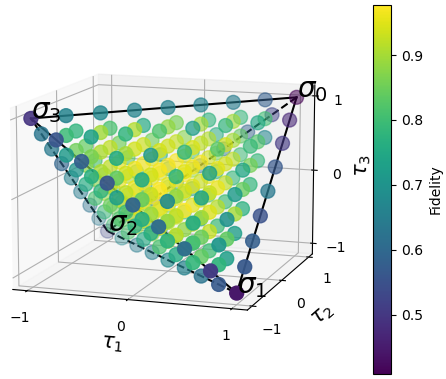
\includegraphics[width=0.45\textwidth]{fidelity-points.png}\\
\caption{Fidelity of one qubit channels using Qiskit's ibmq-lima.}
\end{figure}


\paragraph{$\sigma_3$ parabolic map} $\;$ \\

We take as an example the Pauli dynamical map for one qubit defined as
\begin{eqnarray}
\epsilon(\rho) = \dfrac{1}{4} (1-p)^2 \sigma_0 \rho \sigma_0 + \dfrac{1}{4} (1-p^2) \sigma_1 \rho \sigma_1 + \dfrac{1}{4} (1-p^2) \sigma_2 \rho \sigma_2 + \dfrac{1}{4} (1+p)^2 \sigma_3 \rho \sigma_3 ,
\end{eqnarray}
with $p \in [-1,1]$. \\

To implement this dynamical map using the circuit presented in figure \ref{fig: one-rot-A}, it is necessary to create the state
\begin{eqnarray}
\left(\dfrac{1}{2} (1-p) , \dfrac{1}{2} \sqrt{1-p^2} , \dfrac{1}{2} \sqrt{1-p^2} , \dfrac{1}{2}(1+p) \right)
\end{eqnarray}
on the $2$ ancilla qubits. Luckily, this state can be written in the form $\vec{c} + \vec{a} \cos s + \vec{b} \sin s$ as
\begin{eqnarray}
\begin{pmatrix}
1/2 \\
0 \\ 
0 \\
1/2
\end{pmatrix} + \begin{pmatrix}
0 \\
1/2 \\
1/2 \\
0
\end{pmatrix}  \cos s + \begin{pmatrix}
-1/2 \\
0 \\
0 \\
1/2
\end{pmatrix} \sin s
\end{eqnarray}
with $s = \arcsin p$. According to theorem 1, the fact that the state we need to create over the ancilla qubits can be written like this implies that the dynamical map can be simulated in a quantum computer using only one parametrized rotation. The circuit used will have the same form as that in figure \ref{fig: canal-1qbit-A}, where the part used to create the state on the ancilla qubits will be:
\begin{figure}[h!]
\centering
\begin{quantikz}
\lstick{$aq_0$} & \gate[wires=2]{B} & \ctrl{1} & \gate[wires=2]{A} & \qw \\
\lstick{$aq_{1}$} & & \gate{R_{\sigma_2}(2s)} & & \qw  \\
\end{quantikz}
\caption{Circuit to create 2-qubit state}
\end{figure}

where according to theorem 1, matrices $A$ and $B$ can be chosen as:
\begin{eqnarray}
A &= \begin{pmatrix}
*  & c_0 / \sqrt{1-r^2} & -b_0/r & a_0 /r \\
*  & c_1 / \sqrt{1-r^2} & -b_1/r & a_1 /r \\ 
* & c_2 / \sqrt{1-r^2} & -b_2/r & a_2/r \\
* & c_3 / \sqrt{1-r^2} & -b_3/r & a_3/r \\
\end{pmatrix} = \begin{pmatrix}
0 & 1/\sqrt{2} & -1/\sqrt{2} & 0 \\
-1/\sqrt{2} & 0 & 0 & 1/\sqrt{2} \\
1/\sqrt{2} & 0 & 0 & 1/\sqrt{2} \\
0 & 1/\sqrt{2} & 1/\sqrt{2} & 0
\end{pmatrix} \\
B& = \begin{pmatrix}
0 & 0 & 0 & 1 \\
0 & 1 & 0 & 0\\
0 & 0& 1 & 0 \\
1 & 0 & 0 & 0 
\end{pmatrix}
\end{eqnarray}


To put it to test, we selected $20$ equally spaced values of $p$ between $-0.9$  and $0.9$ and implemented the corresponding circuit using the ibmq-Lima quantum computer. For each point, we used quantum process tomography to obtain the Choi matrix for the channel. Then, we calculated the fidelity of this matrix with respect to the theoretical Choi matrix of the channel. The following figure shows the fidelity of the simulated circuit for each value of $p$.
\begin{figure}[h!]
\centering
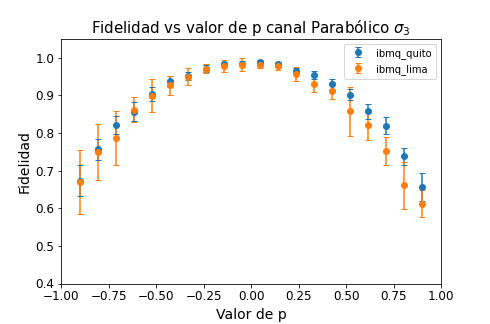
\includegraphics[width=0.55\textwidth]{fidelity-parabolic.PNG} \\
\caption{Fidelity for the Parabolic channel.}
\end{figure}


\newpage
\subsection{Unitary evolution $U = e^{iHt}$}
\section{Exponential maps $e^{iHt}$} % {{{
\label{sec: Exponential maps}
\textbf{Puntos:}
\begin{itemize}
\item We will apply the results about 1PR circuit to another kind of operation, those given by $U  = e^{iHt}$ where $H$ is hermitian  and time independent.
\item \textbf{Lemma:}\textit{ The $n$-qubit operator $U^{iHt}$ can be implemented with a 1PR circuit of $n$ qubits if and only if $D = \text{diag}(e^{i\lambda_0 t}, \cdots, e^{i \lambda_{2^n-1}t})$ can be implemented with a 1PR circuit of $n$ qubits, where $\lambda_j$ are the eigenvalues of $H$.}
\item \textbf{Proof:}  Es b\'asicamente usar que $H = QDQ^{-1}$ para una matriz $Q$ que no depende de $t$ y por lo tanto no agrega compuertas parametrizadas al circuito. 
\item \textbf{Theorem:} \textit{ A n-qubit operator of the form $U = e^{iHt}$ can be implemented using a 1PR circuit if and only if the eigenvalues of $H$ are $-\lambda,0,\lambda$ (for $\lambda$ a real number) and the degeneracies of $\lambda$ and $-\lambda$ are both equal to $2^j$ for some $j\in \{0,1,\cdots,n-1\}$.}
\item \textbf{Proof:} Estoy buscando formas de simplificar la prueba, porque es medio larguita. Pero básicamente es usar el lema y entonces preocuparnos sólo por $D$. Luego  usar el teorema de la sección 3 y notar que sólo hay tres tipos de  $\lambda$s posibles y luego notar que deben de tener esas degeneraciones.
\item \textbf{Proof del regreso:} Aquí quiero recalcar que la prueba es constructiva, ya que consiste en mostrar cómo construir el circuito 1PR que hace la operación a partir de una $H$ que cumpla la hipótesis. 
\item \textbf{Examples.} Mencionar que por el teorema, los ejemplos son sistemas con 3 energías separadas por la misma distancia y con las degeneraciones dadas en el teorema. 
La verdad que no se me ocurren sistemas físicos comunes que cumplan eso.
\begin{itemize}
\item Cualquier matriz $H$ de un qubit cumple el teorema.
\item Cualquier matriz de $n$ qubits que sea el producto tensorial de matrices de Pauli para cada partícula (o sea algo como $\sigma_{i_1} \otimes \sigma_{i_2} \otimes \cdots \otimes \sigma_{i_n}$) cumple el teorema.
\item Estoy viendo para cadenas de espines si hay condiciones para las que cumplan las hipótesis del teorema, pero no he encontrado aún.
\end{itemize}
\item Hice explícitamente el circuito de 2 qubits para $H = \sigma_3 \otimes \sigma_2$ y lo simulé en las computadoras de IBM, obteniendo una fidelidad de $0.85$.
\end{itemize}
% }}}
\newpage

We are now interested on what conditions must an $n$-qubit time independent Hamiltonian $H$
fulfill for the unitary operator $U = e^{iHt}$ to be
implementable with an OPR circuit of $n$ qubits. \\


\textbf{Lemma:} \textit{The $n$-qubit operator $U = e^{iHt}$ can be implemented with an OPR circuit of $n$ qubits
if and only if $D = diag(e^{i\lambda_0 t}, \cdots, e^{i\lambda_{2^n-1}t})$ can be implemented with an OPR circuit of $n$ qubits,
where $\lambda_j$ is the $j$-th eigenvalue of $H$}\\

\textbf{Proof:} The hamiltonian $H$ can be diagonalized as $QHQ^{-1} = diag(\lambda_0,\lambda_1, \cdots,\lambda_{2^n-1})$
 where $Q$ is the  change of  basis matrix and doesn't depend on the parameter $t$ 
 (because $H$ is time independent). Then, the unitary matrix $U = e^{iHt}$ can be diagonalized similarly as $D = QUQ^{-1}$ where $D = diag(e^{i\lambda_0 t}, \cdots, e^{i\lambda_{2^n-1}t})$.
 
Then, if we have an OPR circuit for $U = e^{iHt}$, adding $Q$ and $Q^{-1}$ before and after the circuit converts it into an OPR circuit that
implements $D$. On the other hand, given an OPR circuit for $D$, adding $Q^{-1}$ and $Q$ before and after
converts it into an OPR circuit for $U$. $\blacksquare$. \\


\textbf{Theorem:} \textit{A $n$-qubits operator of the form $U = e^{iHt}$ (where $H$ is time independent) can be implemented 
using an OPR circuit if and only if the eigenvalues of $H$
are $-\lambda, 0, \lambda$ (for $\lambda$ a real number) and the degeneracy of $\lambda$ and $-\lambda$ is $2^j$ for $0 \leq j < n$.} \\

\textbf{Proof:} According to the lemma, if $U = e^{iHt}$ is implementable using an $n$-qubit OPR circuit,
then the diagonal matrix $D = diag(e^{i\lambda_0 t}, \cdots, e^{i\lambda_{2^n-1}t})$ is implementable using an $n$-qubit OPR circuit too,
 where $\lambda_k$ are the eigenvalues of $H$. 

Therefore, according to Property 2 of OPR circuits,
matrix $D$ must have the form $(|\vec{v}_0|, |\vec{v}_1|, \cdots , |\vec{v}_{2^n-1}|)$, 
but because $D$ is diagonal, this form reduces to:
\begin{eqnarray}
D = \begin{pmatrix}
c_{00} + a_{00} e^{is} + b_{00} e^{-is} & 0 & \cdots  \\
0& c_{11} + a_{11} e^{is} + b_{11} e^{-is} & \cdots  \\
 \cdots & \cdots & \ddots 
\end{pmatrix}.
\end{eqnarray}
Furthermore, the column vectors $\vec{a}_j, \vec{b}_j, \vec{c}_j$ must be orthogonal, but because each column has only one nonzero entry,
only one of the vectors can be nonzero, so each entry must be $c_{jj}$ or $a_{jj} e^{is}$ or $b_{jj} e^{-is}$. 
And because the vectors also satisfy $|\vec{a}_j|^2 + |\vec{b}_j|^2 + |\vec{c}_j|^2 = 1$, it must be true that $|c_{jj}|^2 = 1 $
or $|a_{jj}|^2 = 1$ or $|b_{jj}|^2 =1$.
Therefore, the $j$-th entry in the diagonal matrix must be of the form $e^{i \theta_{j}}$ or
$e^{i \theta_{j}} e^{is}$ or $e^{i \theta_j} e^{-is}$. Consequently, we can define the following sets:
\begin{eqnarray}
\Lambda_c = \{\lambda_j  | e^{i\lambda_j t} = e^{i \theta_j}\} \; ,\;
\Lambda_a = \{\lambda_j  | e^{i\lambda_j t} = e^{i \theta_j + is}\} \;,\;
\Lambda_b = \{\lambda_j  | e^{i\lambda_j t} = e^{i \theta_j-is}\}.
\end{eqnarray}
Every eigenvalue must belong to one of these sets. We can prove the following properties of these sets:
\begin{itemize}
\item The only eigenvalues in $\Lambda_c$ are $\lambda_j = 0$: This is because  $e^{i \lambda_j t}  = e^{i \theta_j}$ for every $t$ implies that $\lambda_j = 0$.
\item All eigenvalues in $\Lambda_a$ ($\Lambda_b)$ have the same value:
Take $\lambda_k , \lambda_j \in \Lambda_a (\Lambda_b)$, then $e^{i\lambda_k t} = e^{i \theta_k \pm is} \; ,\; e^{i\lambda_j t} = e^{i\theta_j \pm is}$,
therefore $\lambda_k t = \theta_k \pm s + 2\pi n_k$ and $\lambda_j t = \theta_j \pm s + 2\pi n_j$ with $n_k, n_j$ integers.
 Subtracting these equations implies that $(\lambda_k - \lambda_j)t = \theta_k - \theta_j + 2\pi n_k - 2\pi n_j$. 
 Given that the right side doesn't depend on $t$, we conclude that $\lambda_k - \lambda_j= 0$, so the eigenvalues are the same.
 
\item Eigenvalues in $\Lambda_a$ and $\Lambda_b$ have the same magnitude but opposite sign: 
Take an eigenvalue $\lambda_j \in \Lambda_a$ and $\lambda_k \in \Lambda_b$, 
then just as in the last step, we conclude that $\lambda_jt =  \theta_j + s + 2\pi n_j$ and $\lambda_kt = \theta_k - s + 2\pi n_k$
and adding these equations we get $(\lambda_j+ \lambda_k)t = \theta_j + \theta_k + 2\pi (n_j + n_k)$. 
Given that the right side doesn't depend on $t$, we conclude that $\lambda_j + \lambda_k =0$, so that $\lambda_j$ and $\lambda_k$ have opposite signs but equal magnitude.
\end{itemize}
Therefore, we conclude that the eigenvalues can be chosen out of $H$ must be chosen 3 sets, 
those in $\Lambda_c$ are equal to $0$, those in $\Lambda_a$ are equal to a value we
will call $\lambda$ and those in $\Lambda_b$ are all equal to $-\lambda$. 

Finally, we notice that the degeneracy of $\lambda$ and
$-\lambda$ are $2^j$ for some $j \in \{0, \cdots, n-1\}$.
 To see that, we remember that because it is an OPR circuit, 
Matrix $D$ is equal to $D = A R_{\sigma_3} (2s)B$, 
with $R_{\sigma}$ a rotation applied to the last qubit and controlled by set of the first qubits and $A,B$ 
matrices that don't depend on $s$.
Furthermore, the matrix $R_{\sigma_3}(2s)$ is diagonal and
it has $2^j$ entries equal to $e^{is}$, $2^j$ entries equal to $e^{-is}$ and the rest equal to $1$ 
(where $j+1$ is the number of  control qubits). 
Therefore, we can write $R_{\sigma_3}(2s) = M_1 + e^{is} M_+ + e^{-is} M_-$
 where $M_1, M_+, M_-$ are diagonal matrices with all non-zero entries equal to $1$ and 
$M_+, M_-$ has $2^j$ non-zero entries and $M_1$ has $2^n - 2^{j+1}$ non-zero entries.

Finally, $D = A(M_1 + e^{is} M_+ + e^{-is} M_-) B = AM_1 B + e^{is} AM_+ B + e^{-is} AM_- B$,
and because $D$ is diagonal, $AM_1B , e^{is} AM_+B, e^{-is} AM_- B$ are
diagonal too. Due to the $A$ and $B$ being full-rank matrices, $e^{is} AM_+B$ 
and $e^{-is} AM_-B$ have a rank of $2^j$ and $AM_1B$ has a rank of $2^n- 2^{j+1}$. 
Therefore, considering $D$ is full rank and diagonal, 
$2^j$ of its entries will be $e^{is}$, another $2^j$ will be $e^{-is}$
and the rest will be $1$. \\

\textbf{Constructing the 
Circuit:}  Given that $H$ has the form given in the theorem,
then $e^{iHt}$ can be diagonalized as $D = diag(e^{i\lambda_0 t}, \cdots , e^{i\lambda_{2^n-1}t})$,
where $2^j$ of the entries are $e^{i\lambda t}$, another $2^j$ are $e^{-i\lambda t}$ 
and the rest are $1$. 
Given a value of $j$, we construct a rotation $R_{\sigma_3}(2\lambda t)$ on the last qubit and with $n-1-j$ control qubits 
(whichever we choose, as long as they are $n-1-j$).
Therefore, the matrix representing this rotation is diagonal with $2^j$
entries being $e^{i\lambda t}$, another $2^j$ being $e^{-i\lambda t}$ and the rest being $1$.
This matrix can then be multiplied by matrices that don't depend on $t$
such that the eigenvalues are reordered and we get the matrix $D$.
That it, we can get matrix $D$ using only one rotation that depends on $t$. 
Then, because $U = Q^{-1} D Q$, we can add matrices $Q^{-1}$ and $Q$ to the circuit
to obtain the complete OPR circuit of $U$. $\blacksquare$ \\ 

\textbf{Note:} If we don't care about adding a global phase to the circuit, the eigenvalues can be translated to $-\lambda+a, a, \lambda+a$ for some $a\in \mathbb{R}$.\\

\subsubsection{Example}
\begin{itemize}
\item  Every matrix $H$ of $n$ qubits obtained as the
tensor product of $n$ Pauli operators fulfills the conditions of the theorem, 
because in particular all eigenvalues of $H$ will
be $1$ or $-1$ with the same number of each. 
\item Every matrix $H$ of one qubit fulfills the theorem, since it has two eigenvalues, that can always be written as $-\lambda+a, \lambda+a$.
\item I tried numerically for sums of Pauli matrices. For $2,3$ and $4$ qubits, the sum of two Pauli matrices (formed by the tensor product of $2,3$ or $4$ one qubit Pauli matrices) satisfy the conditions of the theorem.\\
\end{itemize}


\textbf{Example:} Consider $H = \sigma_3 \otimes \sigma_2$ for two qubits. In this case, the hamiltonian matrix is
\begin{eqnarray}
H = \begin{pmatrix}
0 & -i & 0 & 0 \\
i & 0 & 0 & 0 \\
0 &0 & 0 & i \\
0 & 0 & -i & 0
\end{pmatrix}
\end{eqnarray}
that has eigenvalues $\{-1,-1,1,1\}$. This matrix can be diagonalized as
\begin{eqnarray}
Q \begin{pmatrix}
-1 & 0 &0 & 0 \\
0 & -1 &0 & 0 \\
0 & 0 & 1 & 0 \\
0 & 0 & 0 & 1
\end{pmatrix} Q^{\dagger} \;\; ,\;\; Q:= \begin{pmatrix}
-\sqrt{2}/2 & 0 & 0 & - \sqrt{2}/2 \\
\sqrt{2}/2 i & 0 & 0 & -\sqrt{2}/2 i \\
0 &-\sqrt{2}/2 & \sqrt{2}/2 & 0\\
0 &-\sqrt{2}/2 i & -\sqrt{2}/2i & 0
\end{pmatrix},
\end{eqnarray}
therefore, the exponential matrix is given by:
\begin{eqnarray}
U = e^{iHt} = Q \begin{pmatrix}
e^{-it} & 0 &0 & 0 \\
0 & e^{-it} &0 & 0 \\
0 & 0 & e^{it} & 0 \\
0 & 0 & 0 & e^{it}
\end{pmatrix} Q^{\dagger}
\end{eqnarray}
The diagonal matrix between $Q$ and $Q^{\dagger}$ is simply $R_{\sigma_3} (2s)$ applied to the first qubit and without control qubits, therefore
the OPR circuit for this operation is given by figure \ref{fig: 2x3-A}

\begin{figure}
\centering
\begin{quantikz}
\lstick{$q_0$} & \gate[wires=2]{Q^{\dagger}} & \swap{1} & \qw & \swap{1} & \gate[wires=2]{Q} & \qw \\
\lstick{$q_1$} & \qw & \targX{} & \gate{R_Z(2t)} & \targX{}  & \qw & \qw\\
\end{quantikz}
\caption{Circuito para $\sigma_2 \oplus \sigma_3$}
\label{fig: 2x3-A}
\end{figure}
I tried out this circuit on 
real quantum computers for values of $t$ between 
$0$ and $\pi$ and after applying QPT consistently got a fidelity of around $0.85$ for 
every value of $t$.\\

\subsection{Conclusions}
\begin{itemize}
\item
\end{itemize}



\end{document}
